

\graphicspath{{cybernatics/}}

\chapter{Multi-objective Formulation of MSA for Phylogeny Inference}
 Multiple sequence alignment (MSA) is a preliminary task for estimating phylogenies. It is used for homology inference among the sequences of a set of species. Generally, MSA task is handled as a single-objective optimization process.
The alignments computed under one criterion may be different from the alignments generated by other criteria, inferring discordant homologies and thus leading to different hypothesized evolutionary histories relating the sequences. The multi-objective (MO) formulation of MSA has recently been advocated by several researchers, to address this issue. An MO approach independently optimizes multiple (often conflicting) objective functions at the same time and outputs a set of competitive alignments. However, no conceptual or experimental rational from a real-world application perspective has been reported so far for any MO formulation of MSA. This research work investigates the impact of MO formulation in the context of an important scientific problem, namely, phylogeny estimation. Employing popular evolutionary MO algorithms, we show that (a) trees inferred based on alignments produced by the existing MSA methods used in practice are substantially worse in quality than the trees inferred based on the alignments output by an MO algorithm and
(b) even high quality alignments (according to popular measures available in the literature) may fail to achieve acceptable accuracy in generating phylogenetic trees.      
Thus, we essentially ask the following natural question: ``Can a phylogeny-aware (i.e., application-aware) metric guide in selecting appropriate MO formulations to ensure better phylogeny estimation?" Here we report a carefully designed extensive experimental study that positively answers this question. 







\section{Introduction}
\label{sec:introducntion}
Multiple sequence alignment (MSA) task seeks to arrange three or more nucleotide/protein sequences to infer homology, considering various biological phenomena (i.e., evolutionary history, 3D structure etc.). The output is a matrix in which the input nucleotide/protein sequences are the rows and each column (i.e., site) has characters which are homologous which means all those letters descend from the same letter of a common ancestor). The aligned sequences reflect historical substitution, insertion and deletion of genetic materials which are represented as gaps. Accurately recovering these properties through MSA is necessary to accomplish a biological objective such as inferring the evolutionary history relating the sequences known as phylogenetic trees. While computing MSAs, various computational methods and criteria are used to make hypotheses about homology. But the goal of MSA is entirely biological. Figure~\ref{fig:msa_io} illustrates this problem using an example where four hypothetical protein sequences are to be aligned by placing ``necessary'' gaps. In this work, we focus on the MSA tasks in the context of phylogeny estimation which usually functions in two steps. Firstly, the given sequences are aligned using an MSA tool, thereafter a phylogenetic tree is inferred on obtained alignment. The goodness of estimated phylogenetic trees largely rely on the properties of the corresponding alignment. Thus, choosing the ``most appropriate'' MSA method  is important in the phylogenetic context.

\begin{figure}[!htbp]
	\centering
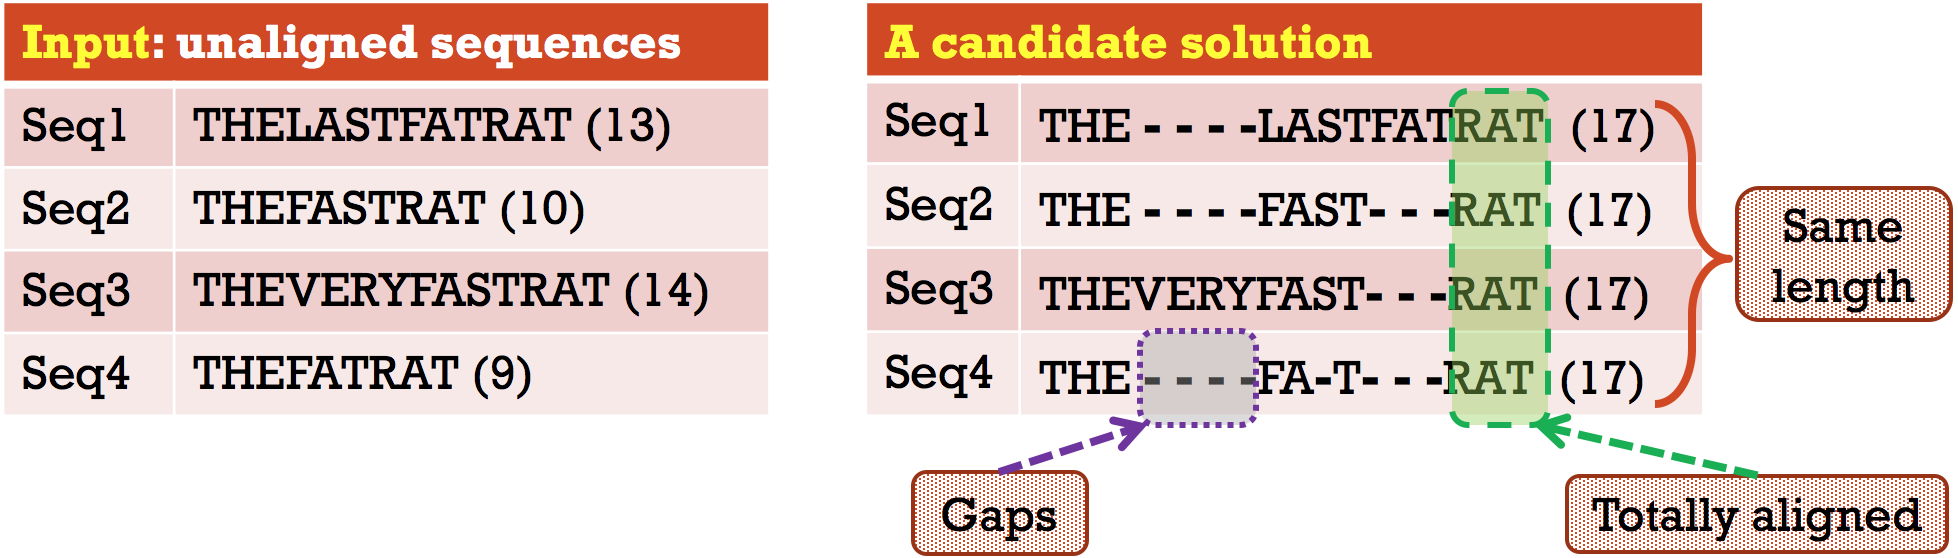
\includegraphics[width=0.6\textwidth]{Figure/msa_io}
\caption{A hypothetical instance of MSA task.} 
		\label{fig:msa_io}
\end{figure}

Previously several researchers (\citep{redelings2005joint, ashkenazy2018multiple}) attempted to improve the phylogeny estimation focusing on MSA computation. While they also agree with our core idea that the nature of MSA computation may influence the outputs (in a domain specific manner) and thereby provided proof of concept. We differ from them by adopting the multi-objective (MO) optimization.
We are motivated from the fact that the alignment generated by optimizing one objective function may be different from the alignments estimated under other objectives. Consequently, this may infer discordant homologies thereby leading to different and often conflicting evolutionary histories relating to the species under consideration. This issue can be addressed by an MO approach that generates a set of alternative alignments by simultaneously optimizing multiple (often conflicting) objectives. But, we are confronted with the challenge of choosing suitable measures/metries to optimize from among a variety of objective functions in literature.
So, we ask the obvious question whether the generic metrics, widely used for assessing the alignment quality, will accurately represent the level of acceptance in the context of a specific application domain, i.e., in our case, phylogeny estimation.
This question has indeed received some discussions, albeit shallow and incomplete, in several studies (\citep{mirarab2015pasta, liu2009rapid}). However, we are not aware of any systematic investigation in the literature to this end. 



This paper, systematically and with scientific rigour, investigates whether a domain-specific performance measure (unlike general-purpose alignment quality measures) can direct us better to find proper MO formulations or tools for MSA when the goal is to infer phylogeny. We suggest a multivariate linear regression based methodology to assess the potential utility of a MO formulation of MSA. Then, following our methodology, we obtained two bi-objective formulations that are capable of yielding better phylogenetic trees than several existing MSA tools.
We perform extensive experimentation with simulated as well as biological datasets and analyze their performance based on quality measures of alignment as well as phylogenetic tree. 
To the best of our knowledge, this is the first work on devising an application-aware MO formulation for tackling MSA. We presented some preliminary results in~\cite{nayeem2019phylogeny}.



\section{Related Works}
\label{sec:literature}
Here we present a concise review of the preceding works relevant to the theme of this study. We concentrate on existing MSA methods along with multi-objective (MO) metaheuristics. For a more comprehensive review, readers can be referred to~\citep{warnow2017computational}.

There exists many methods/tools for computing MSAs in the literature. These methods can be loosely classified into three groups, namely, progressive, consistency-based and iterative methods. Also, many tools combine more than one methods. Progressive method computes the alignment in a ``bottom-up'' fashion by aligning pairs of sequences with the help of a guide tree. It is the basis of numerous MSA methods, including, but not limited to, RetAlign~\citep{szabo2010reticular}, Clustal $\Omega$~\citep{sievers2011fast}, PRANK~\citep{loytynoja2005algorithm}, FSA~\citep{bradley2009fast},  Kalign~\citep{lassmann2008kalign2}, etc. 



A consistency-based method builds a collection of pairwise alignments to aid the generation of an overall accurate alignment. T-Coffee~\citep{notredame2000t}, ProbCons~\citep{do2005probcons}, ProbAlign~\citep{roshan2006probalign} etc. are the representatives of this category. And to attain reliable alignments, the iterative methods attempt to correct the impact of mistakes done at the initial phases by repeating certain critical steps. MAFFT~\citep{katoh2002mafft}, MUSCLE~\citep{edgar2004muscle}, MUMMALS~\citep{pei2006mummals}, ProbCons etc. are some examples of such techniques. Also, we find some ``meta-methods'' in this category, such as, SAT\'e~\citep{liu2009rapid} and PASTA~\citep{mirarab2015pasta}. A tool belonging to this category  co-estimates alignments and phylogenetic trees exploiting existing tools. These are quite popular and widely used in practice. To achieve scalability, they employ a divide-and-conquer approach. The widely accepted way of evaluating the operation of an MSA method is to compare and evaluate the output alignment produced thereby against the reference alignment. Probably the most popular measures used for this purpose are the so called sum-of-pair score (i.e., SP score) and total-column score (i.e., TC score)~\citep{warnow2017computational}. They will be defined shortly in a subsequent section.


The MSA datasets of the current post-genomic era have raised several unprecedented challenges to the scientists. Generally, a default parameter setting is suggested for each MSA method to align any data with reasonable correctness. However, the default configuration cannot assure the best performance across all types of datasets~\citep{rubio2018characteristic}. As an example, a parameter in ProbCons may be cited which controls how many times the refinement passes are done iteratively: while the default value is set to 100, this can vary between zero to 1000. By tuning parameters, better results may be achieved for a particular dataset. Nevertheless, a method cannot beat others across different instances despite having its best parameter setting. 

So we observe the appearance of new methods that combine the strength of different existing tools~\citep{thompson2011comprehensive}. Metaheuristics are one of such methods which can exploit the outputs of different methods to generate superior solutions. The success of such a metaheuristic technique relies on the choice of appropriate optimization objective that is able to help selecting better solutions from among the alternatives and thereby guide the search process towards optimal solutions of MSA. And it is sensible to consider multiple objectives at once as any single one solely cannot effectively address the challenges posed by various datasets. We find that MO techniques are being used effectively to address various real-wold problems in several different domains~\cite{8955943, 9098079, 8984353, 8842602}.
Thus tackling MSA with MO approach is worth investigating.


Recently we notice several works (\citep{da2010alineaga, ortuno2013optimizing, soto2014multi, abbasi2015local, rubio2016hybrid,zambrano2017comparing, rubio2018characteristic}) on the MO formulation for MSA – suggesting upto four objectives to identify and measure the various features of alignment. Maximizing the sum of pairs score may be regarded as the most well-known objective function.
Perhaps the most well-known objective function is the maximization of the sum of pairs score. It evaluates every pair of aligned sequences with the help of a substitution matrix that is expected to represent the dataset traits. Another common  objective to maximize is the totally conserved columns which counts the columns having the same character across all rows. But we know that such columns do not necessarily indicate homology.
Besides, several studies consider minimizing the number of gaps to keep the resultant alignment compact. Also various forms of gap penalties are minimized that adopts a penalization scheme based on gap pattern. Furthermore, entropy and similarity are two minimization objectives which evaluate each column of an alignment. They try to quantify how homogeneous are the letters contain in the same column. It should be noted that, the reference alignment is not allowed to use in the calculation of any objective function. 

We find some unresolved issues in existing studies that advocated the MO formulation of MSA. Firstly, insufficient conceptual or experimental justification for selecting a specific objective to optimize. Next, lack of concrete reasoning for the employment of the two widely accepted performance measures: SP score and TC score. It seems rather reasonable on the contrary that the measures to evaluate the performance should have  reflected the true intent of the MSA task: 
if the purpose is phylogeny inference, then, the success should be evaluated based on a measure that can reliably express the `goodness' and `utility' of the constructed phylogenetic tree. Finally, the dataset used in experimentation, particularly the number of species used therein, is relatively small (i.e., below 50 species).


In this study, our context is phylogeny estimation and we aim to address the above mentioned limitations of MO optimization for MSA in that context. In particular, we propose a new method that leverages multivariate linear regression for selecting application-aware MO formulations. We notice several prior efforts (e.g.,~\citep{lu2012classification, zhou2005study}) on regression-assisted optimization approaches. However, unlike ours, those works focused on constructing a surrogate model, by applying regression techniques, for computationally expensive fitness evaluation.


  \section{Methods}
\label{sec:methods}
Because we deal with numerous objective functions, exisitng MSA methods and datasets, a reader is exposed to an over-preponderance of acronyms and short-cut notations. Therefore, for the sake of ease in exposition and understanding, Table~\ref{tab:acronyms} of the supplementary file alphabetically lists all the acronyms used in this paper along with their intended usage.

\subsection{Experiment settings}
\label{sec:exp_settings}
We summarize Our experimental methodology in six steps as follows.\begin{itemize}
	\item \underline{Step 1:} We identify and choose two bi-objective formulations, effective for phylogeny estimation, by adopting a systematic method incorporating multivariate linear regression analysis with the help of a simulated dataset. \item \underline{Step 2:} We optimize each bi-objective formulation selected in Step 1 by
	 running an appropriate MO metaheuristics on biological datasets. Each run outputs some competitive alignments. 
	\item \underline{Step 3:} Several existing MSA methods are also executed on all these datasets. Each method generates one alignment per dataset.
\item \underline{Step 4:} Based on two measures (i.e., SP and TC scores), that are very popular in the literature, we assess the goodness of all estimated alignments. \item \underline{Step 5:} Employing a standard approach, we infer the phylogenetic tree from every generated alignment. For each of the estimated trees, we assess the goodness thereof in terms of a well-known metric, namely, FN (false negative) Rate~\citep{warnow2017computational}.
	\item \underline{Step 6:} At last, we carefully compare the alignments along with their respective phylogenetic trees generated by the MO approach against those obtained from existing MSA tools. \end{itemize}
\subsection{Objective functions}
\label{sec:formulation}
Most of the real-life optimization problems actually aim to achieve multiple objectives, where objectives are (usually) in conflict with one another. An MO formulation enables us to optimize each objective independently. We select the following three formulations, for this study, considering their simplicity and effectiveness. \begin{itemize}
	\item \textit{\{SOP, TC\} formulation~\citep{da2010alineaga}:} Here, the sum of pairs score (i.e., SOP) and the totally aligned columns (i.e., TC) are maximized. 

	\item \textit{\{Gap, SOP\} formulation~\citep{abbasi2015local}:} Here, SOP is maximized and the number of gaps (i.e., Gap) is minimized.
	
	\item \textit{\{wSOP, TC\} formulation~\citep{rubio2016hybrid}:} Here, wSOP, i.e., the weighted sum of pairs with affine gap penalties and TC are maximized.
\end{itemize}

These objective functions with examples have been discussed in the supplementary file (please check Section~\ref{sec:objective _function}). Here  four new objective functions are proposed in the context of an MSA, which quantify different aspects thereof. We deliberately do not combine multiple aspects of an MSA into a single objective, unlike the approach taken predominantly in the literature. We introduce these four new objective functions as follows: 

\begin{itemize}
	\item \textbf{Minimizing entropy (Entropy)}: Contrary to the usual definition, we consider only non-gap columns for the calculation of entropy.
	
	\item \textbf{Maximizing similarity based on gap containing columns (SimG)}: Here, similarity is calculated only for the columns containing one or more gaps. 
	
	\item \textbf{Maximizing similarity based on non-gap columns (SimNG)}: Here, similarity is calculated only for the columns containing no gap.	
	\item \textbf{Maximizing concentration of gaps (GapCon)}: For each sequence, we count the consecutive gaps and take the mean of these counts. Finally, we average the resultant means for all sequences and use that as the Concentration of gaps.
	
\end{itemize}
At this point a brief discussion on the motivation behind proposing the fourth objective is order. Affine gap penalty~\citep{rani2016multiple} is a widely used objective function that combines (using weighted sum) two aspects of an aligned sequence, namely, the concentration and the number of gaps. Thus, one would need to tune the weight values based on the dataset. To avoid this we decouple the two components/aspects. Notably, the number of gaps (i.e., Gap) has already been considered by us as an objective function. 


From onward, the objectives discussed above are denoted by the acronyms listed in Table~\ref{tab:abbr} . 
\begin{table}[!htbp]
	\centering
\caption{Acronyms used for the optimization objectives.}
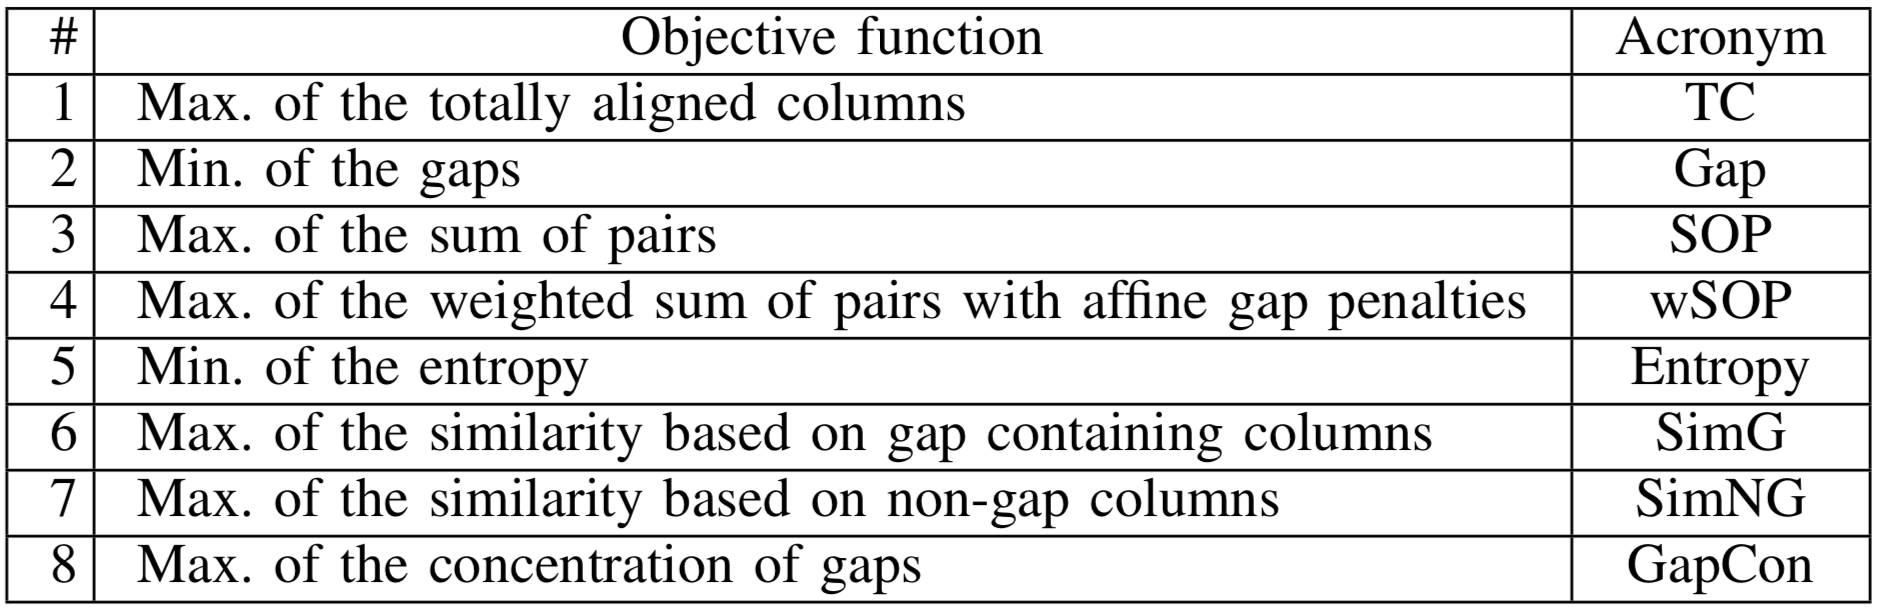
\includegraphics[width=0.6\columnwidth]{Figure/objective_acronym}
	\label{tab:abbr}\end{table}To evaluate SOP and wSOP, a substitution matrix is needed which depends on dataset characteristics. We have employed NUC4.4 and BLOSUM62 (available at ftp://ftp.ncbi.nih.gov/blast/matrices) for nucleotide and protein sequences, respectively. Informatively, all four objective functions we have proposed above are nonparametric.\subsection{MO metaheuristics}
We utilize three well-known MO metaheuristics: NSGA-II~\citep{deb2002fast}, NSGA-III~\citep{deb2014evolutionary} and MOEA/D~\citep{zhang2007moea}. They belong to the class of MO evolutionary algorithms. They start from a set of candidate solutions (termed as population) and then mimics concepts of natural evolution (such as mutation, crossover, selection, etc.) to evolve the population towards the optimal solutions. Unlike single-objective optimization methods, they output a lot of solutions (i.e., members of the final population) which is a compromise among all objectives in the best possible way. Three studies (\citep{zambrano2017m2align, ortuno2013optimizing, zambrano2017comparing}) demonstrated the superiority of NSGA-II to compute MSAs. NSGA-II can effectively tackle problems with upto three objectives whereas NSGA-III is developed in a particular way to handle more than three objectives. Keeping these in minds, we apply them according to Table~\ref{tab:variants}. We run MOEA/D, studied by~\cite{zhu2015novel} for MSA, with one formulation to compare its performance against NSGA-II.
These methods along with important parameters thereof are described in Section~\ref{sec:mop} (of the supplementary file). Besides, a short description of their vital components as follows. 
\begin{itemize}
	\item We used the encoding scheme proposed by~\cite{rubio2016hybrid} which stores each sequence as $[(b_1, e_1),$ $(b_2, e_2), ..., (b_n, e_n)]$, where $(b_i, e_i)$ represents the begin and end position of a group of consecutive gaps in the sequence. \cite{zambrano2017m2align} studied the benefit of such encoding over the traditional binary representation.
	
	\item As mutation operator, we used closed gap shifting~\cite{ortuno2013optimizing}, which randomly chooses consecutive gaps from a sequence and shifts to another random position. This shifting may result in columns having only gaps which are then removed. Thus, in effect, it tries to remove gaps from the MSA. 
	
	\item The crossover operator~\citealp{da2010alineaga} acts as a single-point crossover on two parent alignments (let us refer to them as $ P1 $ and $ P2 $). It picks a random column from P1 to break it into two segments: $ P1^L $ and $ P1^R $. The selected column elements are located in P2 (which are not necessarily belongs to the same column) and used to cut P2 into two segments: $ P2^L $ and $ P2^R $. Then, the generated segments are interchanged between these two parents to create two offspring alignments: [$P1^L + P2^R$] and [$P2^L + P1^R$]. At the end, gaps are used to fill the empty cells (if any) appeared at the junction.
\end{itemize}

We implemented the above two metaheuristics using jMetalMSA~\citep{zambrano2017multi} which is a Java metaheuristic framework for MSA. The important parameters with corresponding values are listed in Table~\ref{tab:parameters}. We adopt the same mutation and crossover operator, along with the associated parameter values, used by~\cite{ortuno2013optimizing}.  

\begin{comment}
We provide a short description of these operators below. 
%publicly available at~\url{https://github.com/jMetal/jMetalMSA}. 

\begin{itemize}

\item The mutation operator is termed as closed gap shifting, where consecutive gaps are randomly chosen and shifted to another random position in a sequence. This shifting may result columns having only gaps which are then removed. Thus this mutation tries to reduce the number of gaps in the MSA. 

\item The crossover operator is the single-point crossover over alignments proposed by~\citealp{da2010alineaga}. The operator randomly selects a column from one parent to split it into two blocks (let us refer to them P1a and P1b). The same selected positions are located in the other parent (which are not necessarily in the same column) and is tailored so that the right piece can be joined to the left piece of the first parent and vice versa (P2a and P2b). Finally, the selected blocks are exchanged between these two parents to create two new individuals with the combination of the blocks: [P1a + P2b] and [P1a + P1b]. After that, any empty space that appears at the junction point is filled with gaps.
%NSGAIII has been shown to perform reasonably on handling a large number of objective functions~\cite{deb2014evolutionary}.	
\end{itemize}
\end{comment}

% Table generated by Excel2LaTeX from sheet 'param'
\begin{table}[!htbp]
	\centering
	\small
	\caption{Major parameters of our algorithms.}
	\begin{tabular}{|c|c|c|} %|c|C{3cm}|C{3.2cm}|
		\hline
		Algo. & \multicolumn{1}{c|}{Parameter} & Value \\
		\hline
		\multirow{5}{*}{All} & Max. generations & 500 \\
		
		\cline{2-3}          & Mutation  & Closed gap shifting \\
		\cline{2-3}          & Mutation rate & 0.2 \\
		\cline{2-3}          & Crossover  & Single-point crossover \\
		\cline{2-3}          & Crossover rate & 0.8 \\ %, $C_r$
		\hline
		\multirow{2}{*}{NSGA-II} & Population size & 100 \\ %, $\overline{N}$
		\cline{2-3}          & No. of runs & 20 \\
		\hline
		\multirow{3}{*}{NSGA-III} & No. of reference points & 120 \\
		\cline{2-3}          & Population size & 120 (78) \\ %, $N$
		\cline{2-3}          & No. of runs & 25 (40) \\
		\hline
		\multirow{2}{*}{MOEA/D} & Population size & 100 \\ %, $\overline{N}$
		\cline{2-3}          & No. of runs & 20 \\
		\cline{2-3}          & Neighborhood size & 10 \\
		\cline{2-3}          & Aggregation function & Tchebycheff approach \\
		\hline
	\end{tabular}%
	\label{tab:parameters}%
\end{table}%

\begin{table}[!htbp]
\centering
	\caption{Selected multi-objective (MO) metaheuristics.}
	\begin{tabular}{|c|l|} \hline
		Algorithm & Objective set to optimize \\
		\hline
		\multicolumn{1}{|c|}{\multirow{2}{*}{NSGA-II}} & \{wSOP, TC\}, 
		\{SOP, TC\},          \\
		& \{Gap, SOP\},
		\{SimG, SimNG\} \\
		\hline
		\multicolumn{1}{|c|}{\multirow{2}{*}{NSGA-III}} & \{wSOP, Gap, TC, SOP\} \\
		& \{SimNG, SimG, GapCon, Entropy, TC, Gap\} \\
		\hline
		\multicolumn{1}{|c|}{\multirow{1}{*}{MOEA/D}} & \{SimNG, SimG\}\\
		\hline
	\end{tabular}\label{tab:variants}\end{table}These algorithms have been implemented using an open-source framework, jMetalMSA (\url{https://github.com/jmetal/jmetalmsa}). We have made our source code available at \url{https://github.com/ali-nayeem/MSA}.\subsection{State-of-the-art MSA tools}
 We use nine representative MSA tools (listed in Table~\ref{tab:msa_tools}) in our experimental study. Each of them is invoked with the default parameter settings. Moreover, we randomly generate the initial population of our chosen metaheuristics by mixing and modifying the alignments generated by these tools. \begin{table}[htbp]
\centering
	\caption{ Existing MSA tools used for experimentation.}
	\begin{tabular}{|l|l||l|l|}
		\hline
		\multicolumn{2}{|c||}{For nucleotide sequences} & \multicolumn{2}{c|}{For protein sequences} \\
		\hline
		\multicolumn{1}{|c|}{Tool} & \multicolumn{1}{c||}{Version} & \multicolumn{1}{c|}{Tool} & \multicolumn{1}{c|}{Version} \\
		\hline
		FSA~\citep{bradley2009fast} & 1.15.9 & FSA   & 1.15.9 \\
		\hline
		PASTA~\citep{mirarab2015pasta} & 1.7.8 & PASTA & 1.7.8 \\
		\hline
		T-Coffee~\citep{notredame2000t} & 11.00 & T-Coffee & 11.00 \\
		\hline
		MAFFT~\citep{katoh2002mafft} & 7.31  & MAFFT & 7.245 \\
		\hline
		Clustal W~\citep{thompson1994clustal} & 2.1   & Clustal W & 2.1 \\
		\hline
		Clustal $ \Omega $~\citep{sievers2011fast} & 1.2.4 & RetAlign~\citep{szabo2010reticular} & 1.0 \\
		\hline
		MUSCLE~\citep{edgar2004muscle} & 3.8.31 & MUSCLE & 3.8.31 \\
		\hline
		PRANK~\citep{loytynoja2005algorithm} & 0.170427 & ProbCons~\citep{do2005probcons} & 1.12 \\
		\hline
		Kalign~\citep{lassmann2008kalign2} & 2.03  & Kalign & 2.04 \\
		\hline
	\end{tabular}\label{tab:msa_tools}\end{table}\subsection{Evaluation of estimated alignments}
\label{sec:msa_eval}
We evaluate estimated alignments using two widely known alignment quality measures: SP and TC scores. They compare the estimated alignment (output) to the reference alignment (reference) in two different ways: the former expresses the ratio of aligned columns recovered in the output with respect to the aligned columns present in the reference, whereas the latter shows the ratio of aligned pairs. 
A higher value implies better score for both of them.\subsection{Estimating Phylogenetic trees}
\label{sec:tree_estimation}
For each generated alignment, we generate the phylogenetic tree. To do so, we use a the standard way of estimating phylogenetic trees from sequence data, i.e., the Maximum Likelihood  method~\cite{liu2011raxml}. FastTree\citep{price2010fasttree} and RAxML~\citep{stamatakis2014raxml} are the most widely used software for this purpose. FastTree can produce output very quickly with negligible difference in tree accuracy compared to RAxML~\cite{liu2011raxml}. In this study we had to estimate numerous phylogenetic trees. So we prefer FastTree over RAxML.\subsection{Evaluating phylogenetic trees}
\label{sec:tree_eval}
We assess and evaluate each of the estimated phylogenetic trees based on the FN Rate against the true phylogenetic tree. 
FN rate actually expresses (in percentage) the fraction of edges that exist in the latter (i.e., in true tree) but are absent in the former (i.e., in the estimated one). Clearly, the smaller the value of FN rate, the more desirable it is. Although there are two more common tree error measures (False Positive (FP rate) and and Robinson-Foulds (RF) rate), all of them are identical when true and estimated trees are binary~\citep{warnow2017computational}. In this study we worked with binary trees only.\subsection{Evaluation of an objective function}
\label{sec:obj_eval}
An MSA objective function should be considered desirable in the context of phylogeny inference only if alignments generated using such objective functions lead to highly accurate phylogenetic trees (i.e., the generate trees exhibit low FN rates).     
Therefore, in an attempt to assess the effectiveness of an objective function we examine how the values thereof are associated with the values of respective FN rates. An objective function is predicted to be a good optimization criteria in our context only if it frequently exhibits positive correlation with FN rate of the trees estimated using the alignments generated by the MO algorithm (leveraging that objective function) for MSA.   
Therefore, in our approach, multivariate linear regression has been employed to estimate the above-mentioned correlation (i.e., regression coefficient) followed by an application of $t$-test (to check the significance of individual regression coefficients) with the null hypothesis that there is no association. While the above regression result may not conclusively indicate the suitability of an objective as an optimization criterion, the chosen objective functions through this methodology can definitely be utilized as potential candidates for further (empirical) validation.



 \section{Results}
\label{sec:results}
This section reports the results of our comprehensive experiments using our methodology and nine existing MSA tools listed in Table \ref{tab:msa_tools}. We start with describing our datasets. In what follows, the (best) results  of an existing MSA method/tool will indicate the results of the nine tools listed in Table \ref{tab:msa_tools}.


\subsection{Datasets}
To conduct our study, we used a simulated dataset (100-taxon simulated dataset~\citep{liu2009rapid}) as well as two biological datasets (biological rRNA datasets~\citep{liu2009rapid} and the BAliBASE 3.0 benchmark~\citep{thompson2005balibase}). The true phylogenetic tree provided with the simulated dataset enables us to analyze whether a MO formulation is potentially application-aware and subsequently we choose two such formulations (Section~\ref{sec:selection_msa_formulation}) which resemble the training period of a supervised learning method to some extent. Afterwards, we evaluate the efficacy of the chosen formulations using biological datasets with respect to the MSA tools listed in Table \ref{tab:msa_tools}.  


From the 100-taxon simulated dataset, we picked five random replicates. And among the biological datasets, we chose two challenging ribosomal RNA datasets along with 27 random BAliBASE instances. We describe these datasets in detail in the supplementary file (Section~\ref{sec:dataset_stat}). 

%\subsection{Dataset statistics}
%\label{sec:dataset_stat}
% Table generated by Excel2LaTeX from sheet 'Sheet1'
\subsubsection{100-taxon simulated dataset}
We used five randomly selected replicates (R0, R4, R9, R14, R19) of simulated nucleotide dataset from the study of~\citealp{liu2009rapid}. It is publicly available at \url{https://sites.google.com/eng.ucsd.edu/datasets/sate-i}. Table~\ref{tab:sim_stat} gives the reference alignment statistics for this dataset.

\begin{table}[htbp]
	\centering
	\caption{Reference alignments for 100-taxon simulated dataset.}
	\begin{tabular}{|l|r|}
		\hline
		\multicolumn{1}{|c|}{Feature} & \multicolumn{1}{c|}{Value} \\
		\hline
		Number of taxa & 100 \\
		\hline
		Number of sites & 1698.2 \\
		\hline
		Percent indels & 40.4 \\
		\hline
		Avg. gap length & 3.1 \\
		\hline
	\end{tabular}%
	\label{tab:sim_stat}%
\end{table}%


\subsubsection{Biological rRNA datasets}
We analyzed two biological ribosomal RNA datasets, 23S.E and 23S.E.aa\_ag, from~\citealp{liu2009rapid} which are challenging for phylogeny estimation methods. Each of these datasets is given with a highly reliable, curated reference alignment from Gutell Lab. The statistics of the reference alignments of these datasets are presented in Table~\ref{tab:bio_stat}. Reference trees for these datasets were generated from the reference alignments by running RAxML~\citep{stamatakis2014raxml} with bootstrapping, and retaining only the highly supported edges. We evaluated generated alignments with respect to the reference alignment using the tool FastSP \citep{mirarab2011fastsp}.
% Table generated by Excel2LaTeX from sheet 'Sheet2'
\begin{table}[htbp]
	\small
	\centering
	\caption{Reference alignments for two biological rRNA datasets.}
	\begin{tabular}{|l|r|r|}
		\hline
		\multicolumn{1}{|c|}{Feature} & \multicolumn{1}{c|}{23S.E.aa\_ag} & \multicolumn{1}{c|}{23S.E} \\
		\hline
		Number of taxa & 144   & 117 \\
		\hline
		Number of sites & 8,619 & 9,079 \\
		\hline
		Percent indels & 61.1  & 59.7 \\
		\hline
		Avg. gap length & 13.5  & 12.6 \\
		\hline
	\end{tabular}%
	\label{tab:bio_stat}%
\end{table}%

\subsubsection{BAliBASE datasets}\label{subsec:balibase_stat}
BAliBASE 3.0 \citep{thompson2005balibase} is the most widely used benchmark alignment databases of protein families. It provides manually refined reference alignments of high quality based on 3D structural superposition. These datasets are organized into six groups according to their families and similarities: RV11 (very divergent sequences, residue identity below 20\% ), RV12 (medium to divergent sequences, 20\%-40\% residue identity), RV20 (families with one or more highly divergent sequences), RV30 (divergent subfamilies), RV40 (sequences with large terminal N/C extensions), and RV50 (sequences with large internal insertions). In this study, we selected four to five representative datasets from each group as reported in Table~\ref{tab:balibase}. We generated reference trees for these datasets by running RAxML~\citep{stamatakis2014raxml} with bootstrapping. We evaluated estimated alignments with respect to the core blocks (regions for which reliable alignments are known to exist) using the program bali\_score available at~\url{http://www.lbgi.fr/balibase/BalibaseDownload/}.

% Table generated by Excel2LaTeX from sheet 'Sheet2'
\begin{table}[htbp]
	\small
	\centering
	\caption{ BAliBASE datasets selected for this study.}
	\begin{tabular}{|l|l|}
		\hline
		\multicolumn{1}{|c|}{Group} & \multicolumn{1}{c|}{Datasets selected} \\
		\hline
		RV11  & BB11005, BB11018, BB11020, BB11033 \\
		\hline
		RV12  & BB12001, BB12013, BB12022, BB12035, BB12044 \\
		\hline
		RV20  & BB20001, BB20010, BB20022, BB20033, BB20041 \\
		\hline
		RV30  & BB30002, BB30008, BB30015, BB30022 \\
		\hline
		RV40  & BB40001, BB40013, BB40025, BB40038, BB40048 \\ %
		\hline
		RV50  & BB50001, BB50005, BB50010, BB50016 \\
		\hline
	\end{tabular}%
	\label{tab:balibase}%
\end{table}%

\subsection{Selection of appropriate MO formulations}
\label{sec:selection_msa_formulation}
As we stated above, our simulated dataset is used to find out potentially ``application-aware'' MO formulation(s). Through extensive experimentation, We first choose a bi-objective formulation from among three popular MO formulations found in the literature (see Section \ref{sec:methods}). Subsequently, we propose a new promising bi-objective formulationfrom among four objectives proposed in this study (see Section \ref{sec:methods}). In each case, we follow a systematic approach based on two criteria: (1) the selected two objectives should be conflicting to each other, (2) the selected objectives should exhibit a relatively good association with the FN rate. Note that, criterion (1) makes the employment of an MO algorithm more attractive as a compromise between two conflicting objectives increases the diversity of generated solutions. 
\begin{comment}
\begin{figure*}[!htbp]    
\begin{adjustwidth}{-1cm}{-1cm}
\centering
\begin{subfigure}{0.35\textwidth}
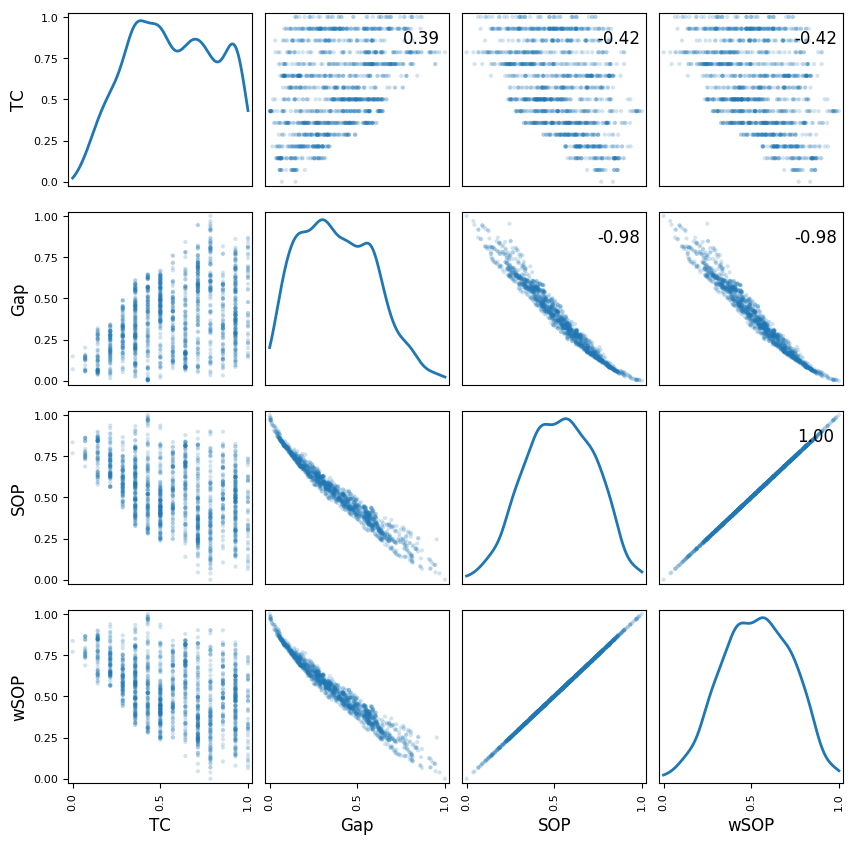
\includegraphics[width=\columnwidth]{Figure/NumGaps_SOP_TC_wSOP/precomputedInit/R0/fig/scatter_mattrix}
\caption{R0}
\end{subfigure}    
\begin{subfigure}{0.35\textwidth}
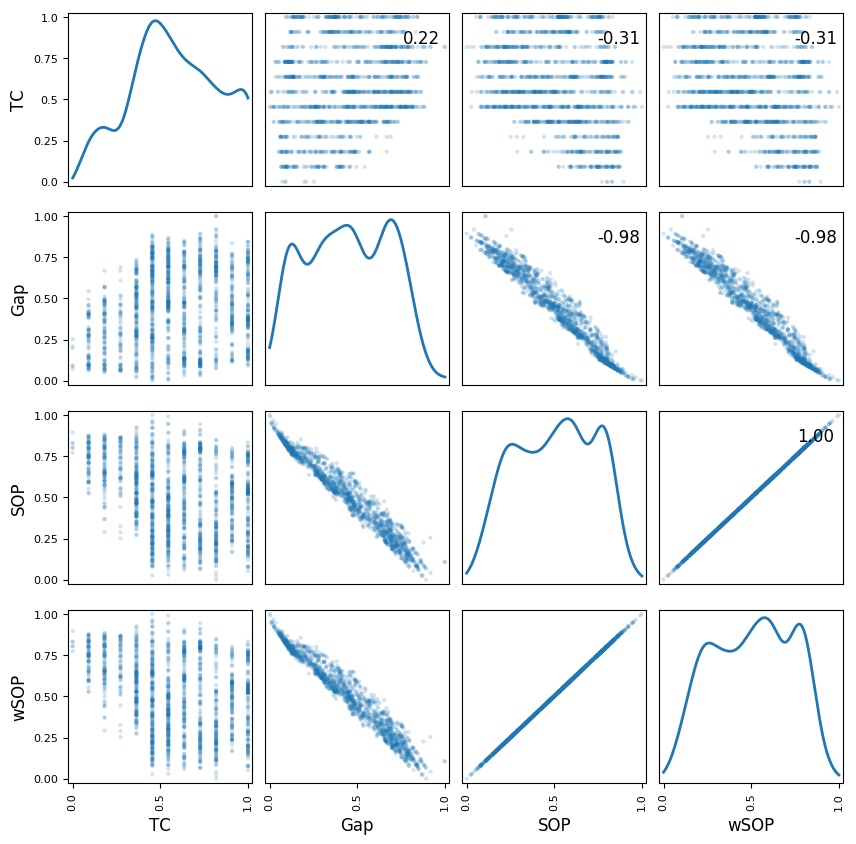
\includegraphics[width=\columnwidth]{Figure/NumGaps_SOP_TC_wSOP/precomputedInit/R4/fig/scatter_mattrix}
\caption{R4}
\end{subfigure}
\begin{subfigure}{0.35\textwidth}
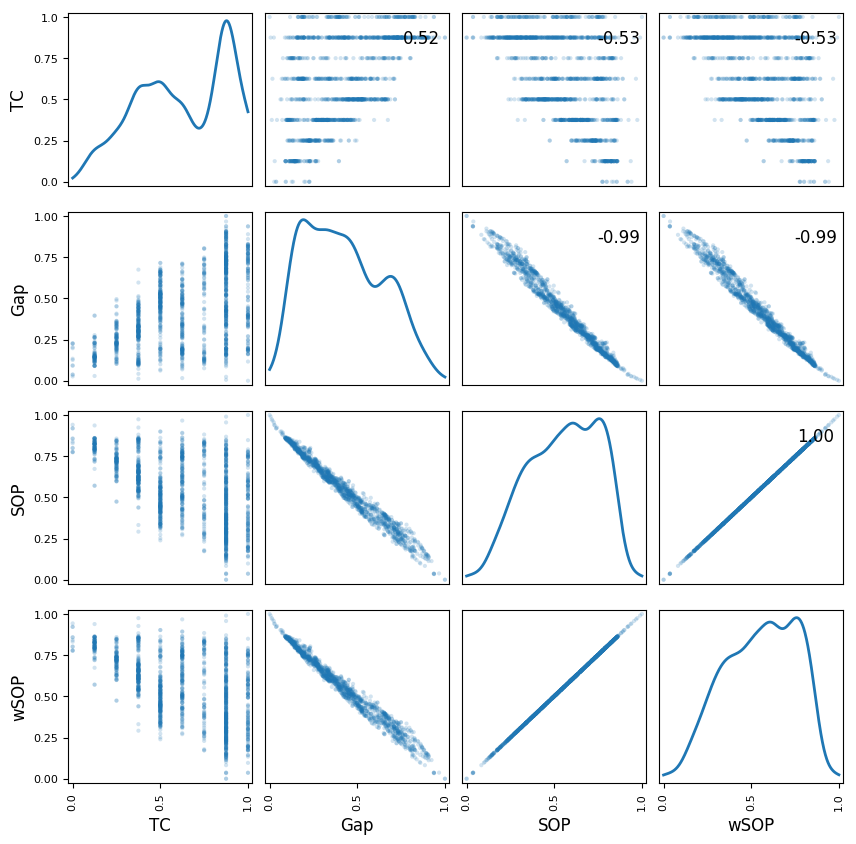
\includegraphics[width=\columnwidth]{Figure/NumGaps_SOP_TC_wSOP/precomputedInit/R9/fig/scatter_mattrix}
\caption{R9}
\end{subfigure}
\begin{subfigure}{0.35\textwidth}
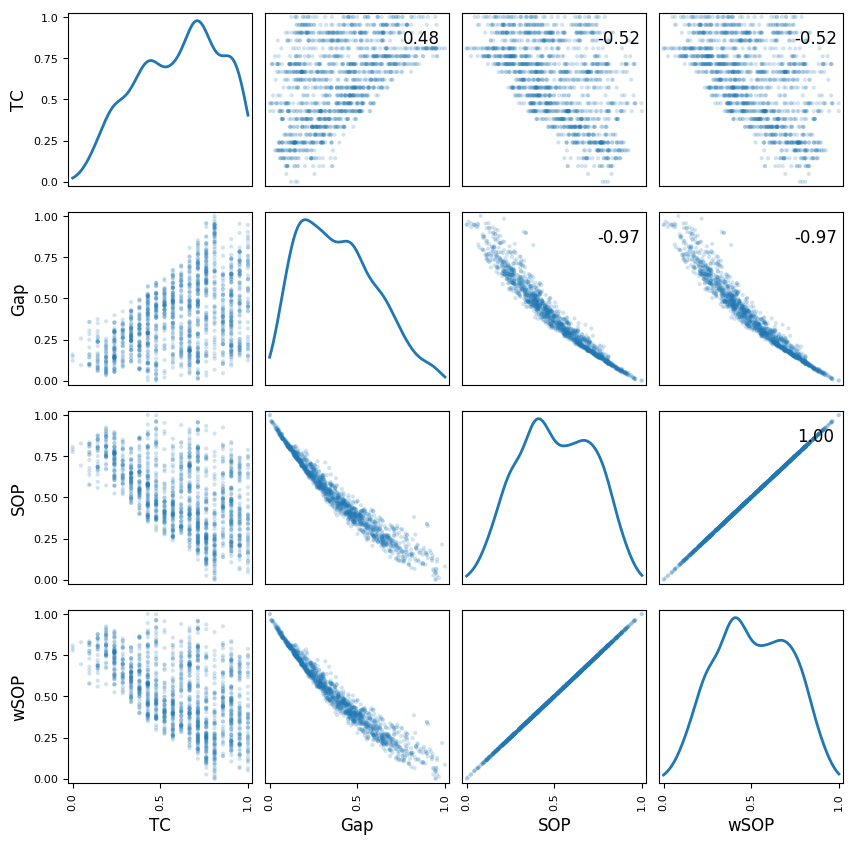
\includegraphics[width=\columnwidth]{Figure/NumGaps_SOP_TC_wSOP/precomputedInit/R14/fig/scatter_mattrix}
\caption{R14}
\end{subfigure}
\begin{subfigure}{0.35\textwidth}
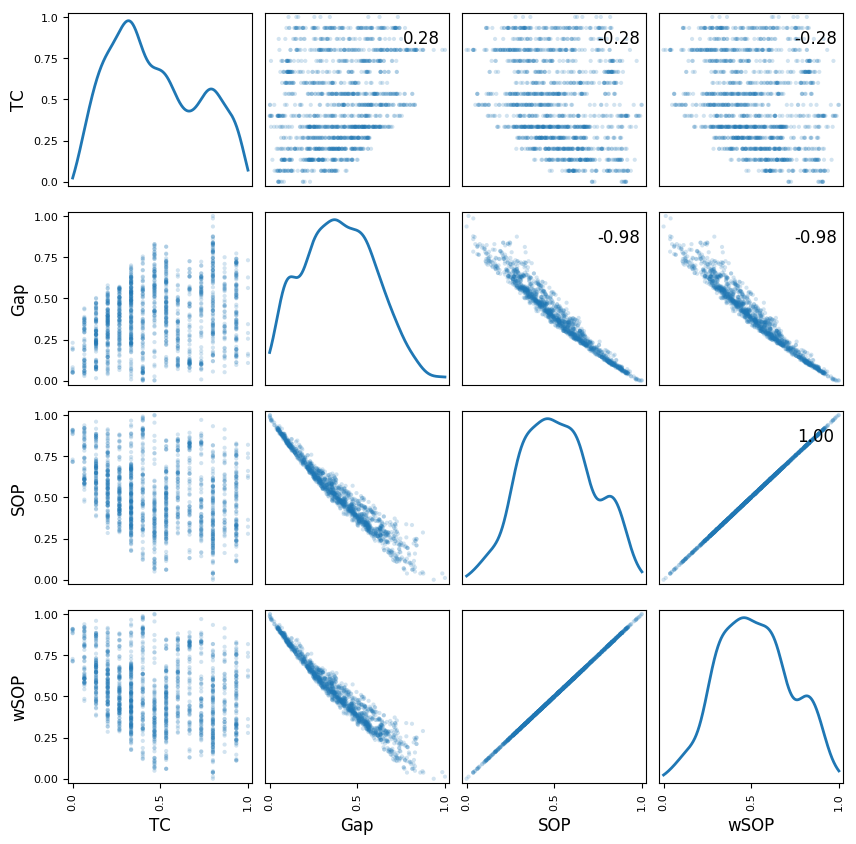
\includegraphics[width=\columnwidth]{Figure/NumGaps_SOP_TC_wSOP/precomputedInit/R19/fig/scatter_mattrix}
\caption{R19}
\end{subfigure}
\caption{\underline{100-taxon simulated dataset:} Scatter-plot matrices depicting the pairwise relationship of all objective functions on five randomly selected replicates. We turn each objective function into minimization form and then normalize using min-max technique. In each matrix, the diagonal cells show the distribution of objective values (estimated using KDE) while the non-diagonal cells show the correlation between pairs of objective functions. Each upper-diagonal cell contains the value of correlation coefficient $r$ of the corresponding pair of objective functions.}
\label{fig:nature_obj}
\end{adjustwidth}
\end{figure*}

\begin{figure*}[!htbp]
\centering
\small
\begin{adjustwidth}{-1cm}{-1cm}
\begin{tabular}{l||C{0.24\textwidth}|C{0.24\textwidth}|C{0.24\textwidth}|C{0.24\textwidth} }
& TC & Gap & SOP & wSOP\\\hline\hline
\rotatebox[origin=c]{-90}{R0} & 
\raisebox{-.5\height}{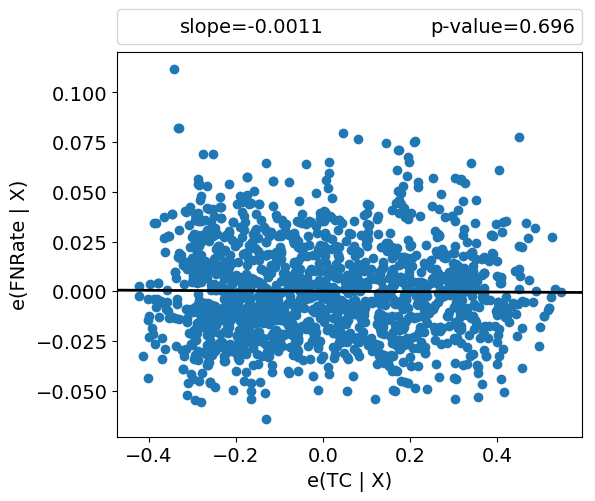
\includegraphics[width=0.25\textwidth]{Figure/NumGaps_SOP_TC_wSOP/precomputedInit/R0/fig/tc_partial_regression}} &
\raisebox{-.5\height}{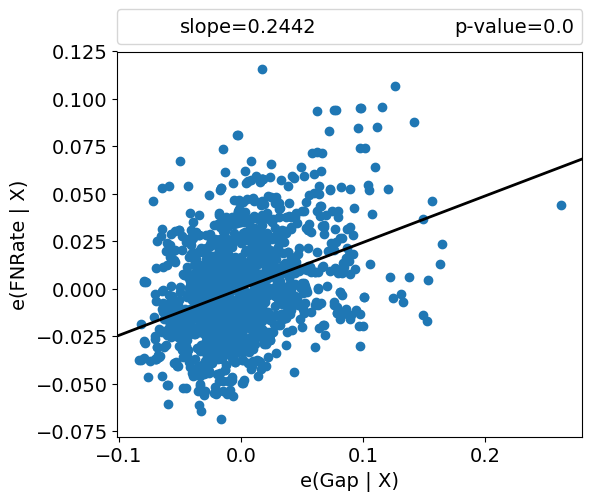
\includegraphics[width=0.25\textwidth]{Figure/NumGaps_SOP_TC_wSOP/precomputedInit/R0/fig/gap_partial_regression}} & 
\raisebox{-.5\height}{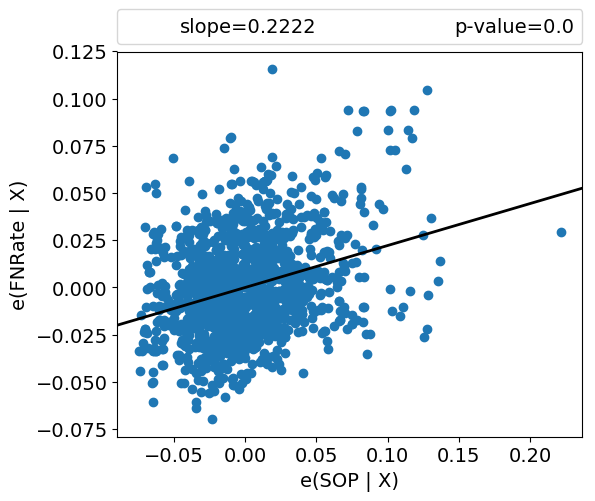
\includegraphics[width=0.25\textwidth]{Figure/NumGaps_SOP_TC_wSOP/precomputedInit/R0/fig/sop_partial_regression}} & 
\raisebox{-.5\height}{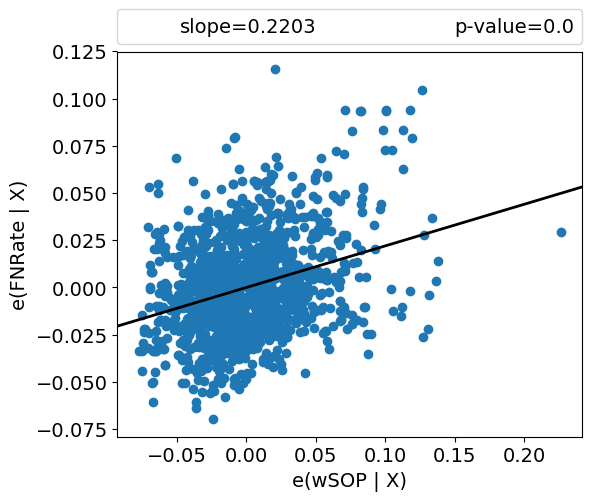
\includegraphics[width=0.25\textwidth]{Figure/NumGaps_SOP_TC_wSOP/precomputedInit/R0/fig/wsop_partial_regression}}     
\\\hline
\rotatebox[origin=c]{-90}{R4} &
\raisebox{-.5\height}{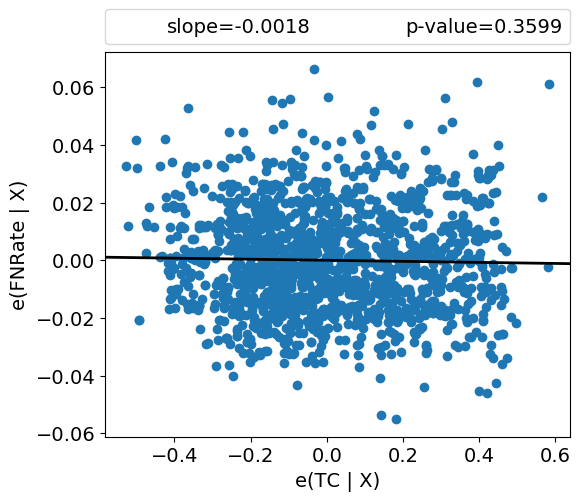
\includegraphics[width=0.25\textwidth]{Figure/NumGaps_SOP_TC_wSOP/precomputedInit/R4/fig/tc_partial_regression}} &
\raisebox{-.5\height}{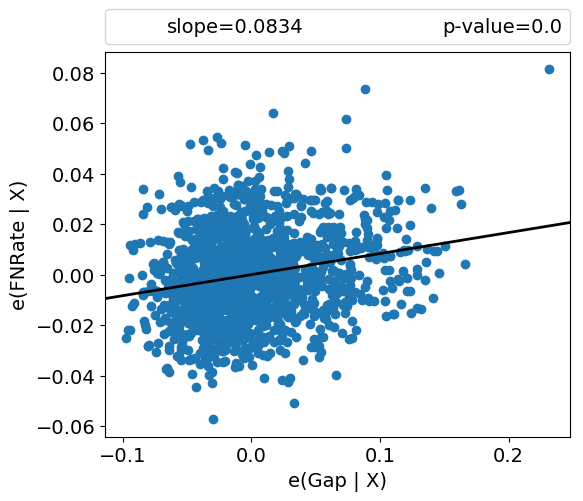
\includegraphics[width=0.25\textwidth]{Figure/NumGaps_SOP_TC_wSOP/precomputedInit/R4/fig/gap_partial_regression}} & 
\raisebox{-.5\height}{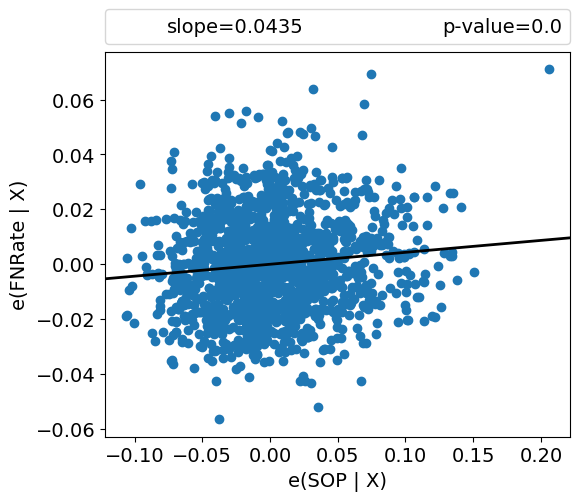
\includegraphics[width=0.25\textwidth]{Figure/NumGaps_SOP_TC_wSOP/precomputedInit/R4/fig/sop_partial_regression}} & 
\raisebox{-.5\height}{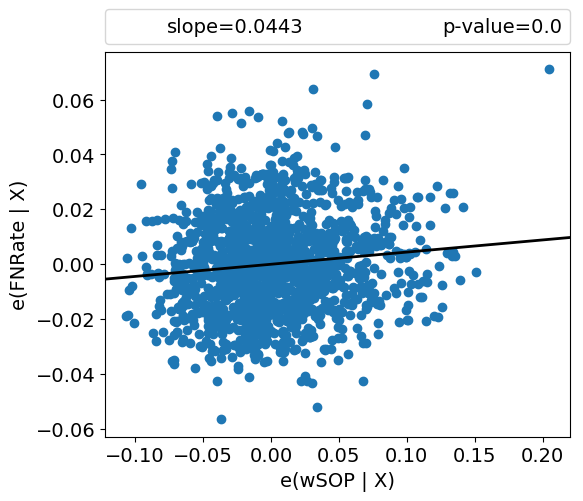
\includegraphics[width=0.25\textwidth]{Figure/NumGaps_SOP_TC_wSOP/precomputedInit/R4/fig/wsop_partial_regression}}
\\\hline
\rotatebox[origin=c]{-90}{R9} &
\raisebox{-.5\height}{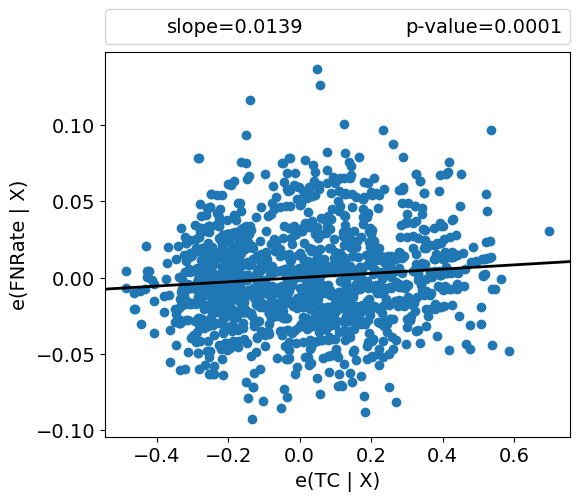
\includegraphics[width=0.25\textwidth]{Figure/NumGaps_SOP_TC_wSOP/precomputedInit/R9/fig/tc_partial_regression}} &
\raisebox{-.5\height}{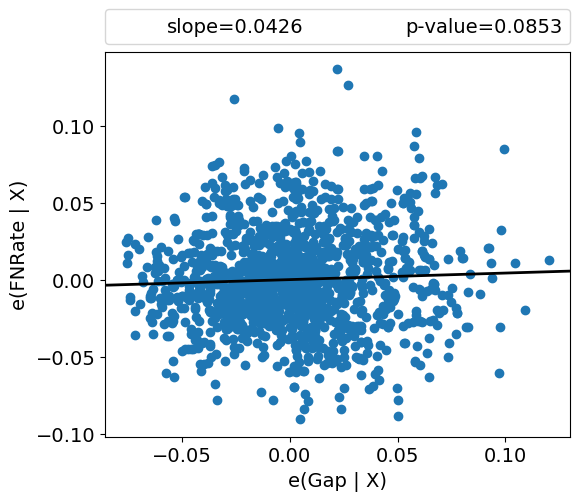
\includegraphics[width=0.25\textwidth]{Figure/NumGaps_SOP_TC_wSOP/precomputedInit/R9/fig/gap_partial_regression}} & 
\raisebox{-.5\height}{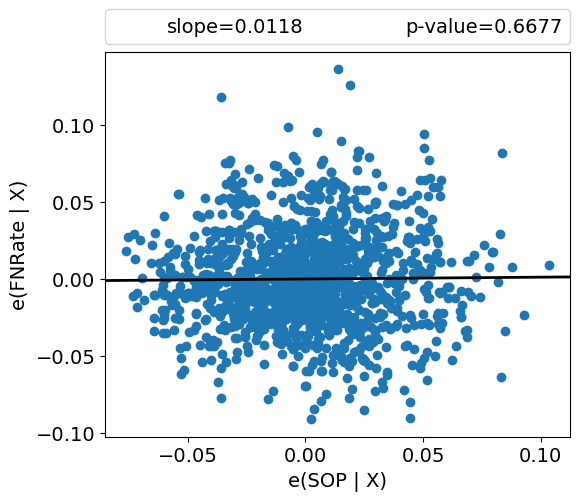
\includegraphics[width=0.25\textwidth]{Figure/NumGaps_SOP_TC_wSOP/precomputedInit/R9/fig/sop_partial_regression}} & 
\raisebox{-.5\height}{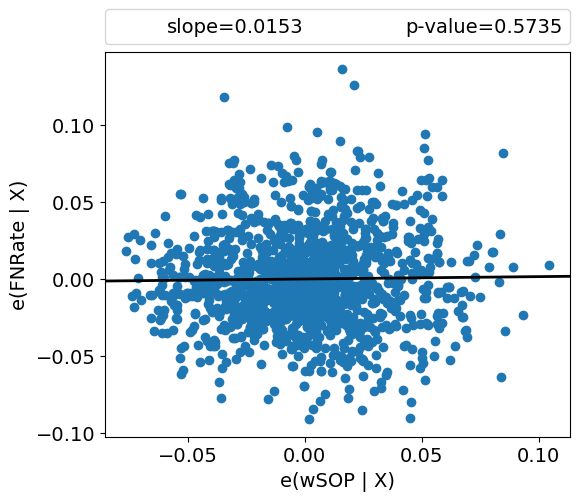
\includegraphics[width=0.25\textwidth]{Figure/NumGaps_SOP_TC_wSOP/precomputedInit/R9/fig/wsop_partial_regression}}
\\\hline
\rotatebox[origin=c]{-90}{R14} &
\raisebox{-.5\height}{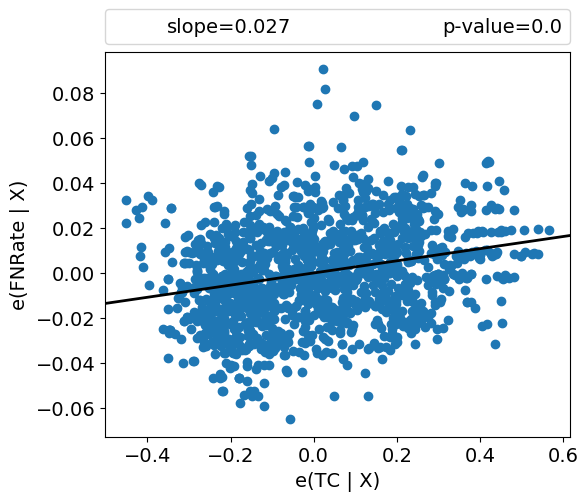
\includegraphics[width=0.25\textwidth]{Figure/NumGaps_SOP_TC_wSOP/precomputedInit/R14/fig/tc_partial_regression}} &
\raisebox{-.5\height}{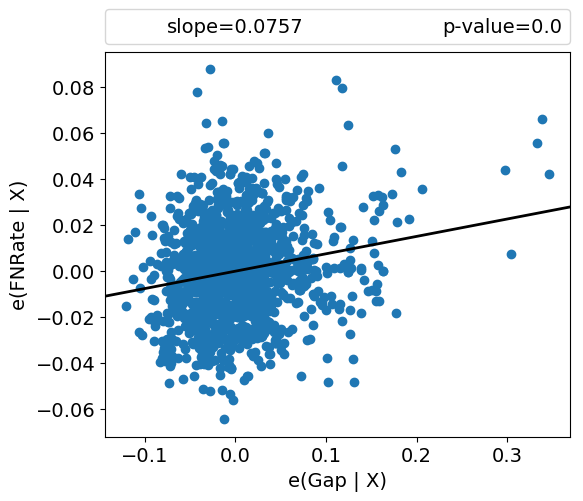
\includegraphics[width=0.25\textwidth]{Figure/NumGaps_SOP_TC_wSOP/precomputedInit/R14/fig/gap_partial_regression}} & 
\raisebox{-.5\height}{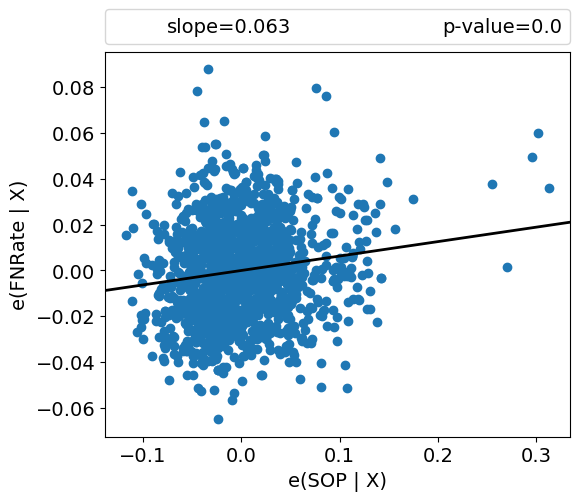
\includegraphics[width=0.25\textwidth]{Figure/NumGaps_SOP_TC_wSOP/precomputedInit/R14/fig/sop_partial_regression}} & 
\raisebox{-.5\height}{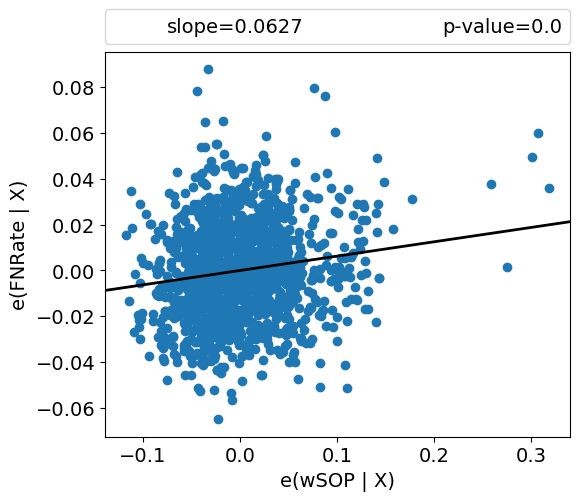
\includegraphics[width=0.25\textwidth]{Figure/NumGaps_SOP_TC_wSOP/precomputedInit/R14/fig/wsop_partial_regression}}
\\\hline
\rotatebox[origin=c]{-90}{R19} &
\raisebox{-.5\height}{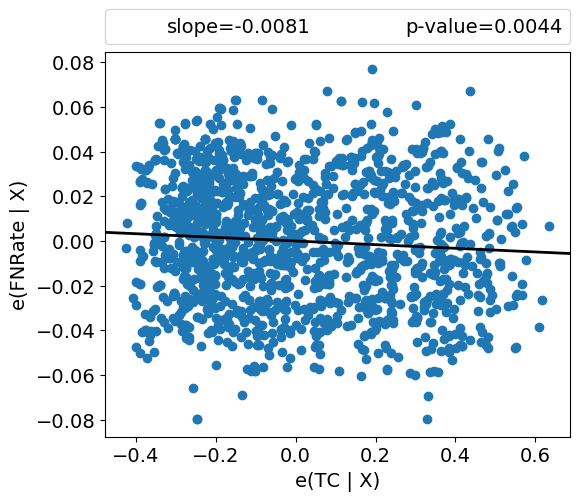
\includegraphics[width=0.25\textwidth]{Figure/NumGaps_SOP_TC_wSOP/precomputedInit/R19/fig/tc_partial_regression}} &
\raisebox{-.5\height}{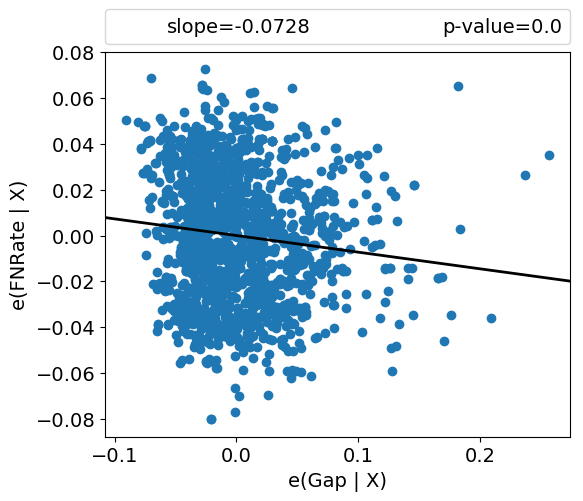
\includegraphics[width=0.25\textwidth]{Figure/NumGaps_SOP_TC_wSOP/precomputedInit/R19/fig/gap_partial_regression}} & 
\raisebox{-.5\height}{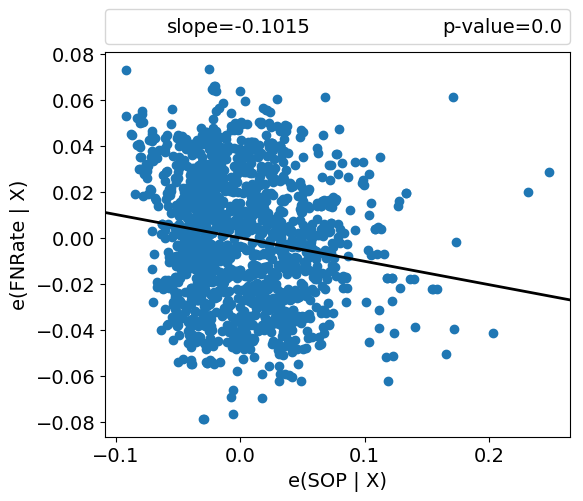
\includegraphics[width=0.25\textwidth]{Figure/NumGaps_SOP_TC_wSOP/precomputedInit/R19/fig/sop_partial_regression}} & 
\raisebox{-.5\height}{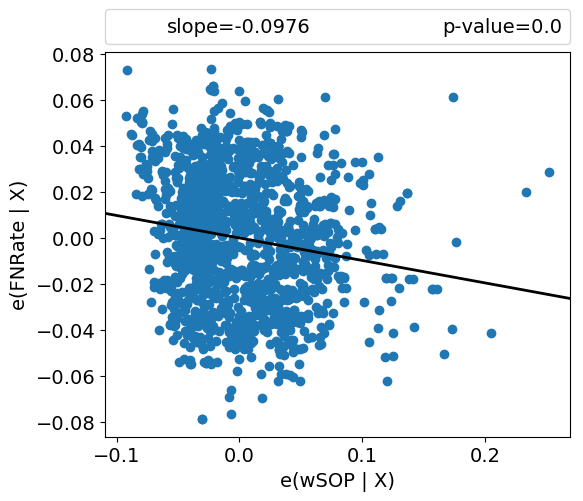
\includegraphics[width=0.25\textwidth]{Figure/NumGaps_SOP_TC_wSOP/precomputedInit/R19/fig/wsop_partial_regression}}
\\\hline
\end{tabular}
\caption{\underline{100-taxon simulated dataset:} Multiple linear regression model for identifying the association among FN rate and three objective functions (TC, Gap and SOP/wSOP) fitted to five randomly selected replicates. There is one figure for each possible combination (replicate, objective function). Each partial regression plot shows the association between an objective function and FN rate while holding the remaining two objectives constant. In a plot for an objective function $ OF $, the horizontal axis, $e(OF|X)$, denotes the residuals from regressing $OF$ against the remaining objective functions and the vertical axis, $e(FNRate|X)$, denotes the residuals from regressing FN rate against all the objective functions except $ OF $.} 
\label{fig:mul_lin_reg}
\end{adjustwidth}
\end{figure*}

\begin{figure*}[!htbp]
\centering
\begin{adjustwidth}{-1cm}{-1cm}
\begin{subfigure}{0.22\textwidth}
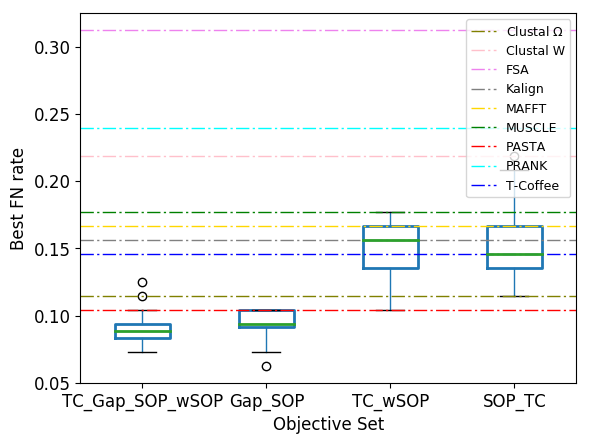
\includegraphics[width=\columnwidth]{Figure/summary/precomputedInit/R0/objset_fnrate_rank}
\caption{R0}
\end{subfigure}    
\begin{subfigure}{0.22\textwidth}
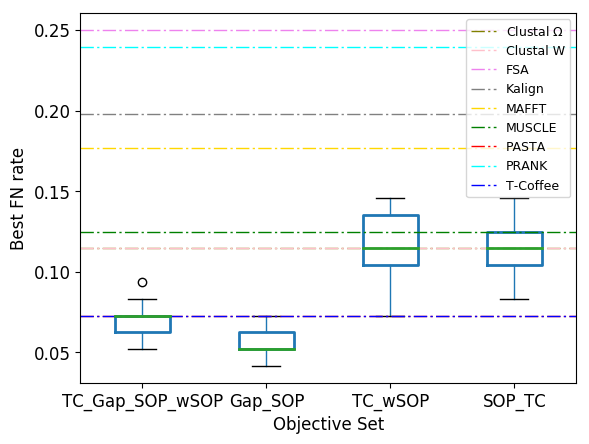
\includegraphics[width=\columnwidth]{Figure/summary/precomputedInit/R4/objset_fnrate_rank}
\caption{R4}
\end{subfigure}
\begin{subfigure}{0.22\textwidth}
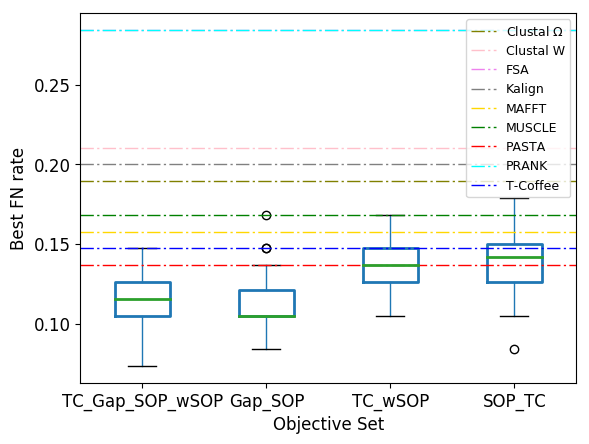
\includegraphics[width=\columnwidth]{Figure/summary/precomputedInit/R9/objset_fnrate_rank}
\caption{R9}
\end{subfigure}
\begin{subfigure}{0.22\textwidth}
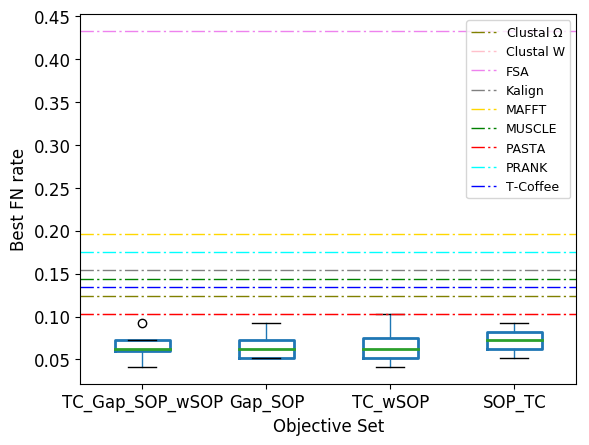
\includegraphics[width=\columnwidth]{Figure/summary/precomputedInit/R14/objset_fnrate_rank}
\caption{R14}
\end{subfigure}
\begin{subfigure}{0.22\textwidth}
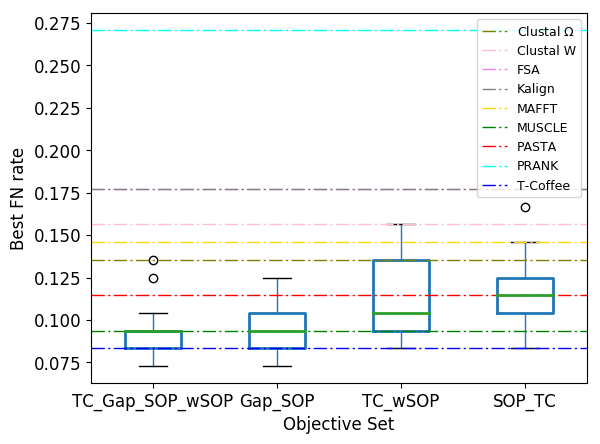
\includegraphics[width=\columnwidth]{Figure/summary/precomputedInit/R19/objset_fnrate_rank}
\caption{R19}
\end{subfigure}
\caption{\underline{100-taxon simulated dataset:} Comparison among objective sets based on the distribution of the collection of the best FN rates from each run. The performance of the state-of-the-art tools are shown using horizontal lines.}
\label{fig:rank_best_fn_rate}
\end{adjustwidth}
\end{figure*}
\end{comment}

\subsubsection{Selecting from three chosen formulations from the literature}
\label{sec:existing_msa_formulation}
To reduce computational burden we carefully study the MO formulations from the literature and pre-select three from among those to focus our research thereon. So we select one from among the three formulations from Table~\ref{tab:abbr} of Section~\ref{sec:methods}. 
Five replicates, namely, R0, R4, R9, R14 and R19, are selected randomly for this experimentation. 



To conduct multivariate linear regression analysis, we need a large pool of diverse alignments. So we run NSGA-III~\citep{deb2014evolutionary} to optimize all objectives (i.e., \{Gap, SOP, wSOP, TC\}) independently for 25 times and combine unique solutions output by each run. Figure~\ref{fig:nature_obj} in the supplementary file presents a $ 4\times4 $ scatter-plot matrix showing the pairwise relationship among all the objectives from this collection. Here we derive the following two important observations.
\begin{enumerate}
	
	\item SOP is entirely correlated with wSOP across all replicates. So optimizing both of them is redundant. Moreover, this high level of correlation causes multicollinearity, a serious trouble in regression analysis~\citep{montgomery2012introduction}. Hence, in the regression model, we will not consider this pair of objectives simultaneously.  
	
	\item Clearly SOP is conflicting with Gap in all cases. So by optimizing them together, many diverse solutions can be generated due to a compromise between these two objectives~\citep{kalyanmoy2001multi}. Such a diverse collection is expected to contain desirable alignment across a variety of datasets.
	
\end{enumerate}

We see inter-dependency among the objective values. Therefore, to avoid getting any spurious result, we want to estimate the correlation between a particular objective function and FN rate keeping the rest of the objectives constant~\citep{montgomery2012introduction}. We accomplish this with the help of the regression model as follows:
\begin{equation}
\small
\begin{split}
\text{FN rate} = \beta_0 + \beta_1 \times \text{TC}+ \beta_2 \times \text{Gap} + 
\beta_3 \times \text{SOP (or wSOP)} + \epsilon \label{eq:multi_lin_reg}
\end{split}
\end{equation}
Here $\epsilon$ is a Gaussian error component with zero mean and some fixed standard deviation. And each coefficient except $\beta_0$ (i.e., the intercept) shows the expected variation in the False Negative rate (i.e., FN rate) per unit variation in the respective objective, rest of the objectives remaining constant. That is why, $\beta_1, \beta_2$ and $\beta_3$ are termed as partial regression coefficients.  
We learn the values of these coefficients (i.e., slopes) using the least-squares method (illustrated using Figure~\ref{fig:mul_lin_reg} in the supplementary file) based on the data (i.e, objective values and FN rates) obtained from the alignments produced by the optimizing of \{Gap, SOP, wSOP, TC\} by NSGA-III. Also, we test the significance of association by applying $t$-test on individual coefficient  $\beta_i$ (with null hypothesis $\beta_i=0$). These regression results allow us to derive two interesting points as follows.
\begin{enumerate}
	\item Gap, SOP and wSOP exhibit better correlation with FN rate (having p-value $<$ 0.05 indicating 95\% confidence) compared to other objective functions in most of the replicates (R0, R4 and R14). So, they are expected to lead towards alignments that can yield better phylogenetic trees.
	\item No objective shows any considerable association in case of R4 and R19 which indicates that an objective might not perform equally across different datasets. 
\end{enumerate}
Next we would like to assess the performance of these MO formulations in terms of FN rate. So for each bi-objective formulation, we independently run NSGA-II~\citep{deb2002fast} 20 times and infer phylogenetic trees for all generated alignments. We have presented the variation of best FN rates collected from each run in a figure in the supplementary file (Figure~\ref{fig:rank_best_fn_rate}). In what follows, We discuss some key observations:
\begin{enumerate}
	\item Naturally giving more objectives to an MO metaheuristics increase its probability of finding the best solution. So we see that the unified formulation \{TC, Gap, SOP, wSOP\} often shows superior performance over the bi-objective formulations. However, in this study, we have preferred smaller MO formulations to reduce the overall complexity.
\item \{Gap, SOP\} achieves better FN rates compared to other bi-objective formulations. And its performance is very close to \{TC, Gap, SOP, wSOP\}. This finding conforms the outcome of our regression analysis pointed before.
	\item Both \{Gap, SOP\} and \{TC, Gap, SOP, wSOP\} can consistently outperform the state of the art tools in terms of FN rate.
\end{enumerate}
Based on our experimental results presented above, we can rate \{Gap, SOP\} as the most appropriate among our pre-selected formulations from literature. 


\subsubsection{Selecting a new formulation}
\label{sec:new_msa_formulation}
From the results discussed so far, one may assume that an objective is more desirable if it exhibits a better correlation with the corresponding FN rate.  
So, we try to form a new objective set as follows. As detailed in Section~\ref{sec:formulation}), firstly, we propose four new objective functions, namely, Entropy, SimG, SimNG and GapCon, each of which, quantifies one particular aspect of MSA. We now run NSGA-III in order to optimize the combined objective set, \{Entropy, TC, Gap, SimG, SimNG, GapCon\} (i.e., we include TC and Gap as well), for 40 times thereby generating numerous diverse alignments.
We then employ multivariate linear regression to analyze and assess the correlations between our proposed objective functions and corresponding FN rates (please check Figure~\ref{fig:new_nature_obj} in the supplementary file for a visualization). In what follows we present our key observations in this regard.
\begin{itemize}
	\item Entropy is strongly correlated with SimG which poses an issue in our multiple regression analysis. Therefore, these two objectives should not remain together in our in our regression model; nor should they be combined in the MO formulation.
	
	\item We witness a conflicting relationship between SimG and SimNG. Therefore, through a simultaneous optimization of these two objectives, a MO metaheuristic can expect to generate a (large) number of alignments that are diverse.
\end{itemize}

Now we use the following model to express as well as capture the relationship between the proposed objective functions and the corresponding FN rates:
\begin{equation}
\small
\begin{split}
\text{FN rate} = \beta_0 + \beta_1 \times \text{SimNG}+ \beta_2 \times \text{GapCon} + 
\beta_3 \times \text{SimG (or Entropy)} + \epsilon \label{eq:new_multi_lin_reg}
\end{split}
\end{equation}
Now, the regression coefficients are estimated by fitting the model of Equation \ref{eq:new_multi_lin_reg} to the data (i.e., objective values and FN rates) obtained from a diverse collection of alignments generated by optimizing \{Entropy, TC, Gap, SimG, SimNG, GapCon\}, i.e., the combined objective set. In the sequel, we notice that, both SimG and SimNG exhibit a positive correlation with FN rate. Hence, the objective set \{SimG, SimNG\} is chosen. In the supplementary file, we have presented a visualization using partial regression plots (Figure~\ref{fig:new_mul_lin_reg}).


\subsubsection{Selection mechanism}%{Selection of appropriate multi-objective formulations}
\textit{(The following should be read in conjunction with the description presented in Section~\ref{sec:selection_msa_formulation} of the main text)} 

We visualize the interrelations among the objective values of the solutions, obtained by running NSGA-III to optimizes the objective set \{Gap, SOP, wSOP, TC\} on five randomly selected replicates (R0, R4, R9, R14, R19) of 100-taxon simulated dataset, using a $ 4\times4 $ scatter-plot matrix~\cite{kalyanmoy2001multi} as shown in Figure~\ref{fig:nature_obj}. Here each diagonal cell of a matrix depicts the distribution of the values of an objective function estimated using kernel density estimation which is a non-parametric way to estimate the probability density function of a random variable. And the non-diagonal cells show the correlation between each pair of objective functions. As our evolutionary algorithms tries to minimize all objective functions, we treat the maximization objective values by multiplying with -1. In the sequel, we normalize all the objective values using min-max technique and as such the maximization objectives are turned into minimization ones.

We estimate the coefficients of multiple linear regression model associating FN rate with each of the objective function from \{Gap, SOP, wSOP, TC\} using least-squares method and illustrate them using partial regression plots~\citep{montgomery2012introduction} in Figure~\ref{fig:mul_lin_reg}. We apply $t$-test on individual regression coefficient (i.e., slope) $\beta_i$ (with null hypothesis $\beta_i=0$) to test the significance of that association. The test results (slope, $p$-value) are incorporated in the figure.

We measure the strength of each objective set based on the FN rate achieved by the members of generated solution set. To accomplish this, For each set of objective functions, we run NSGA-II~\citep{deb2002fast} for 20 times following the standard practice of operations research (OR) literature (due to the stochastic nature of metaheuristics). Each run generates a set of solutions that represents the trade-offs in satisfying all objectives. Afterwards, we inferred ML tree for each of the generated alignment. We collected the best FN rates from each of the 20 solution sets and describe the distribution of these FN rates using boxplots which are shown in Figure~\ref{fig:rank_best_fn_rate}. In these boxplots we also incorporate the FN rates achieved by the state-of-the-art tools for comparison using horizontal lines.

\begin{figure*}[!htbp]	
	\begin{adjustwidth}{-1cm}{-1cm}
		\centering
		\begin{subfigure}{0.35\textwidth}
			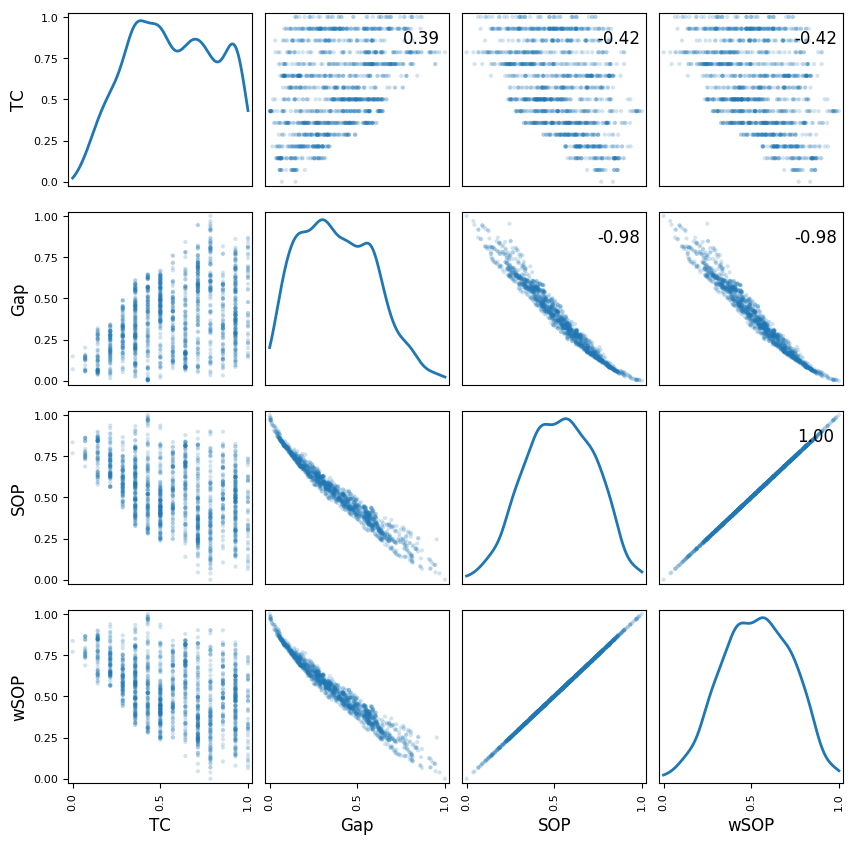
\includegraphics[width=\columnwidth]{Figure/NumGaps_SOP_TC_wSOP/precomputedInit/R0/fig/scatter_mattrix}
			\caption{R0}
			%\label{fig:con_pr09}
		\end{subfigure}	
		\begin{subfigure}{0.35\textwidth}
			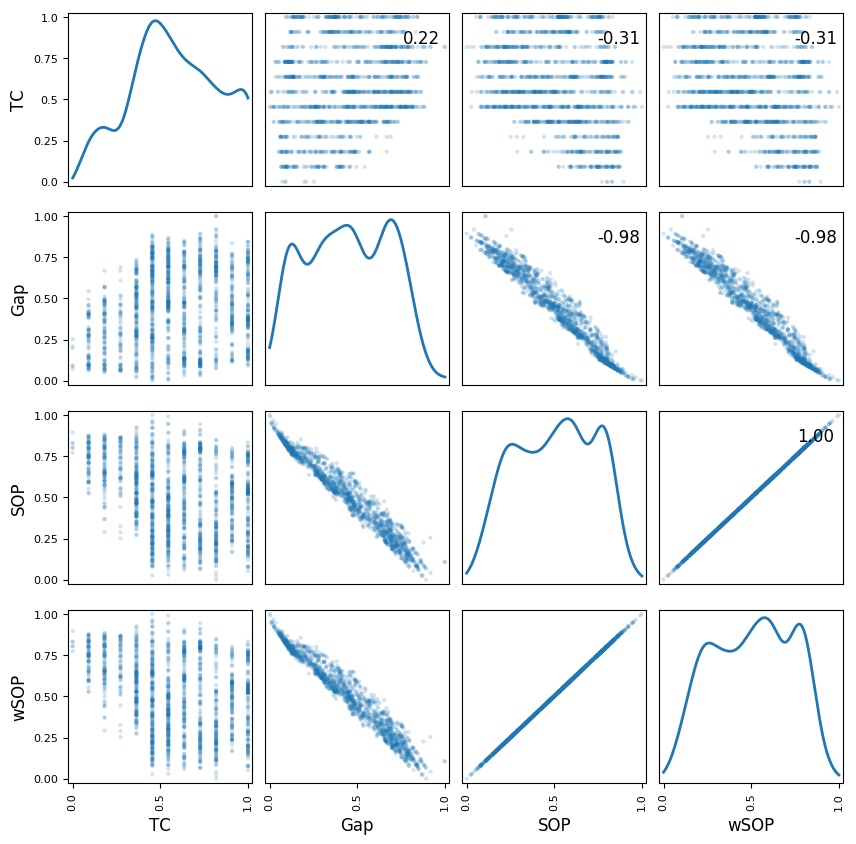
\includegraphics[width=\columnwidth]{Figure/NumGaps_SOP_TC_wSOP/precomputedInit/R4/fig/scatter_mattrix}
			\caption{R4}
			%\label{fig:con_pr09}
		\end{subfigure}
		\begin{subfigure}{0.35\textwidth}
			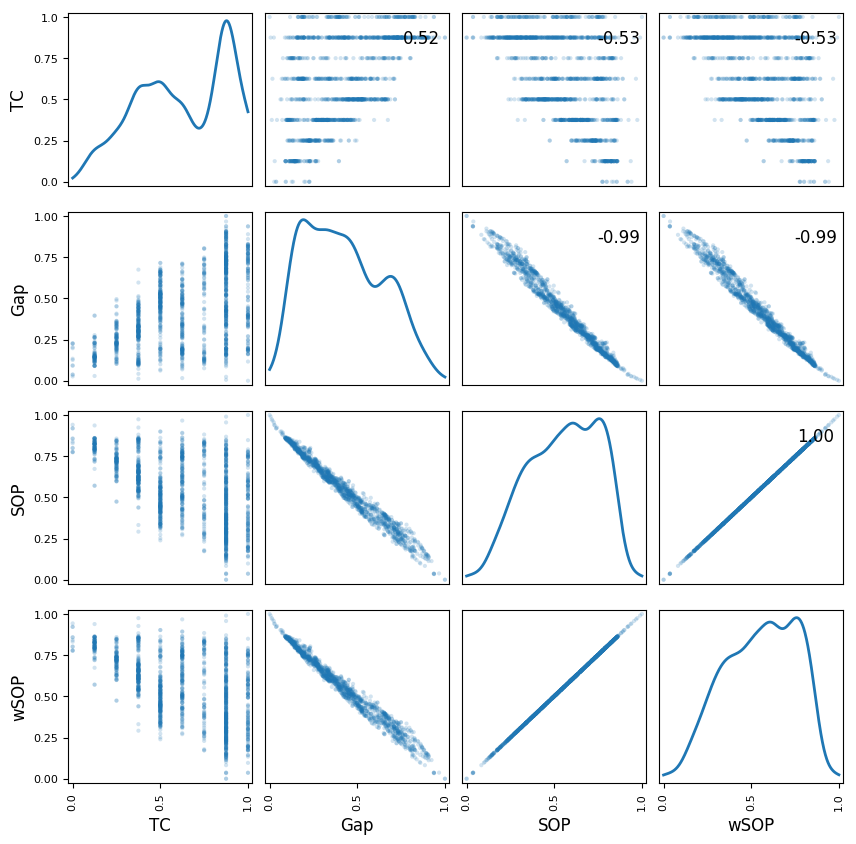
\includegraphics[width=\columnwidth]{Figure/NumGaps_SOP_TC_wSOP/precomputedInit/R9/fig/scatter_mattrix}
			\caption{R9}
			%\label{fig:con_pr09}
		\end{subfigure}
		\begin{subfigure}{0.35\textwidth}
			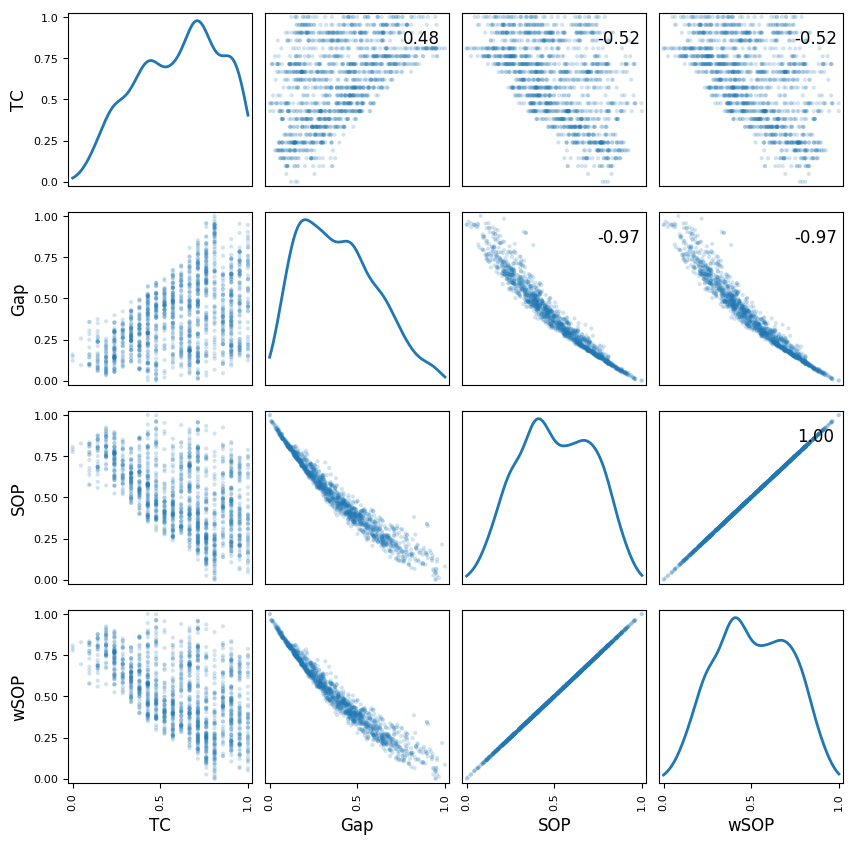
\includegraphics[width=\columnwidth]{Figure/NumGaps_SOP_TC_wSOP/precomputedInit/R14/fig/scatter_mattrix}
			\caption{R14}
			%\label{fig:con_pr09}
		\end{subfigure}
		\begin{subfigure}{0.35\textwidth}
			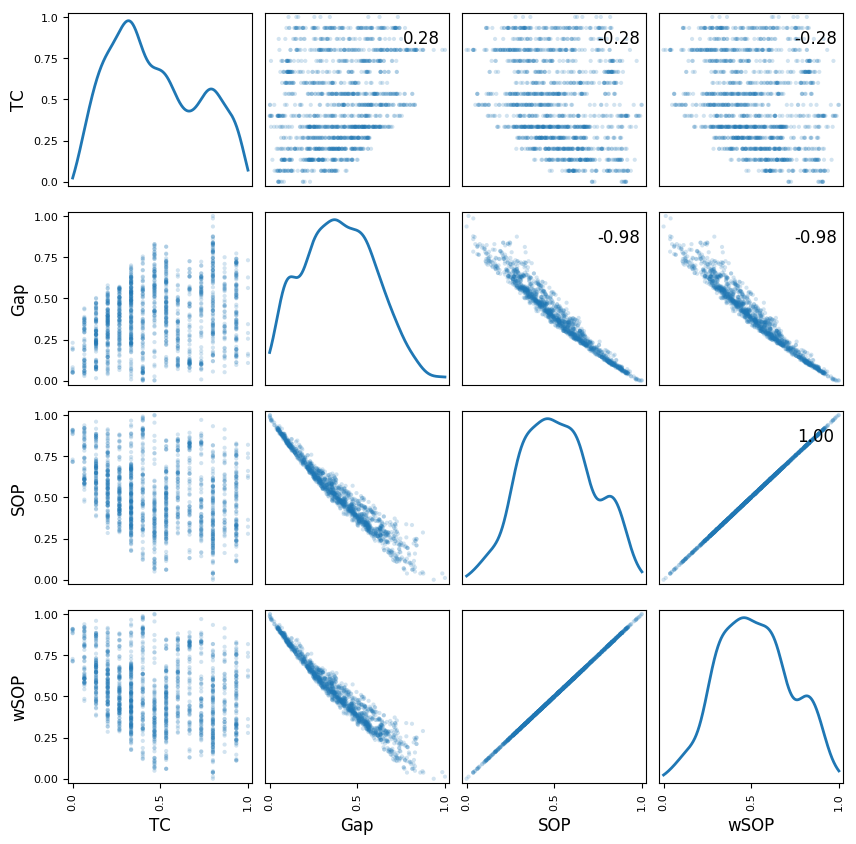
\includegraphics[width=\columnwidth]{Figure/NumGaps_SOP_TC_wSOP/precomputedInit/R19/fig/scatter_mattrix}
			\caption{R19}
			%\label{fig:con_pr09}
		\end{subfigure}
		\caption[Scatter-plot matrices for four objective functions on 100-taxon simulated dataset]{\underline{100-taxon simulated dataset:} Scatter-plot matrices depicting the pairwise relationship of all objective functions on five randomly selected replicates. We turn each objective function into minimization form and then normalize using min-max technique. In each matrix, the diagonal cells show the distribution of objective values (estimated using kernel density estimation which is a non-parametric way to estimate the probability density function of a random variable) while the non-diagonal cells show the correlation between pairs of objective functions. Each upper-diagonal cell contains the value of correlation coefficient $r$ of the corresponding pair of objective functions.}
		\label{fig:nature_obj}
	\end{adjustwidth}
\end{figure*}

\begin{figure*}[!htbp]
	\centering
	\small
	\begin{adjustwidth}{-1cm}{-1cm}
		\begin{tabular}{l||C{0.24\textwidth}|C{0.24\textwidth}|C{0.24\textwidth}|C{0.24\textwidth} }
			& TC & Gap & SOP & wSOP\\\hline\hline
			\rotatebox[origin=c]{-90}{R0} & 
			\raisebox{-.5\height}{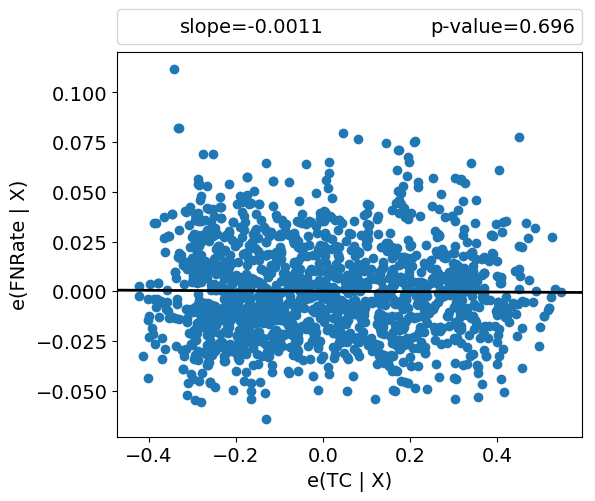
\includegraphics[width=0.22\textwidth]{Figure/NumGaps_SOP_TC_wSOP/precomputedInit/R0/fig/tc_partial_regression}} &
			\raisebox{-.5\height}{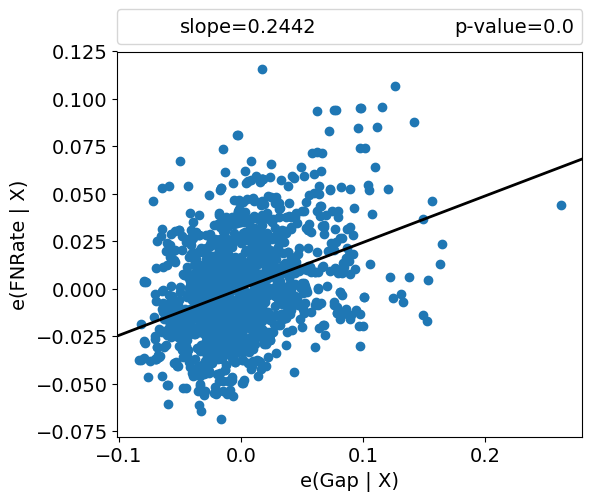
\includegraphics[width=0.22\textwidth]{Figure/NumGaps_SOP_TC_wSOP/precomputedInit/R0/fig/gap_partial_regression}} & 
			\raisebox{-.5\height}{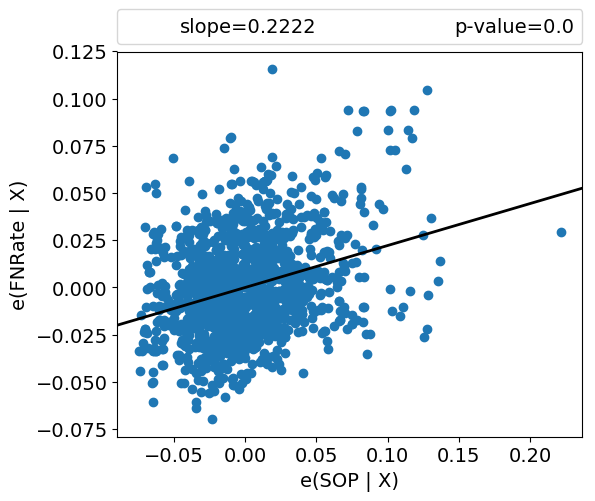
\includegraphics[width=0.22\textwidth]{Figure/NumGaps_SOP_TC_wSOP/precomputedInit/R0/fig/sop_partial_regression}} & 
			\raisebox{-.5\height}{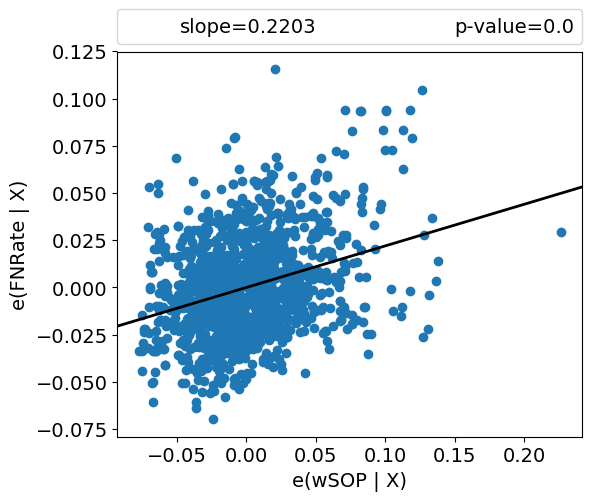
\includegraphics[width=0.22\textwidth]{Figure/NumGaps_SOP_TC_wSOP/precomputedInit/R0/fig/wsop_partial_regression}} 	
			\\\hline
			\rotatebox[origin=c]{-90}{R4} &
			\raisebox{-.5\height}{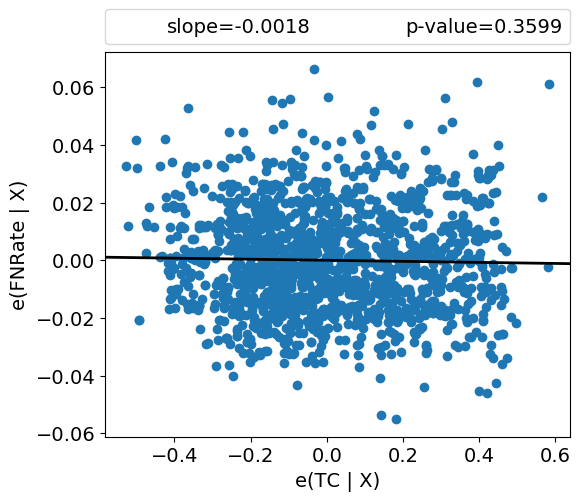
\includegraphics[width=0.22\textwidth]{Figure/NumGaps_SOP_TC_wSOP/precomputedInit/R4/fig/tc_partial_regression}} &
			\raisebox{-.5\height}{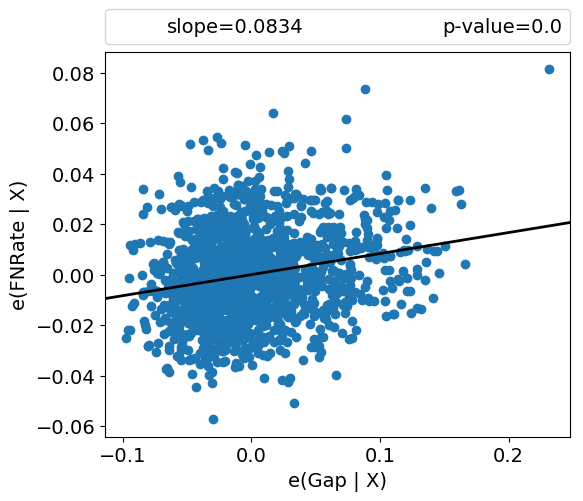
\includegraphics[width=0.22\textwidth]{Figure/NumGaps_SOP_TC_wSOP/precomputedInit/R4/fig/gap_partial_regression}} & 
			\raisebox{-.5\height}{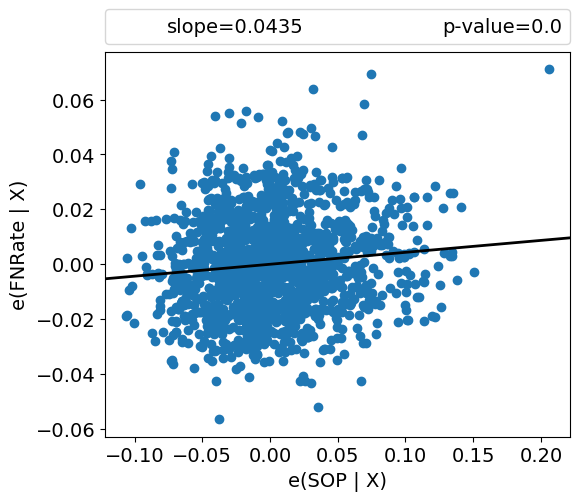
\includegraphics[width=0.22\textwidth]{Figure/NumGaps_SOP_TC_wSOP/precomputedInit/R4/fig/sop_partial_regression}} & 
			\raisebox{-.5\height}{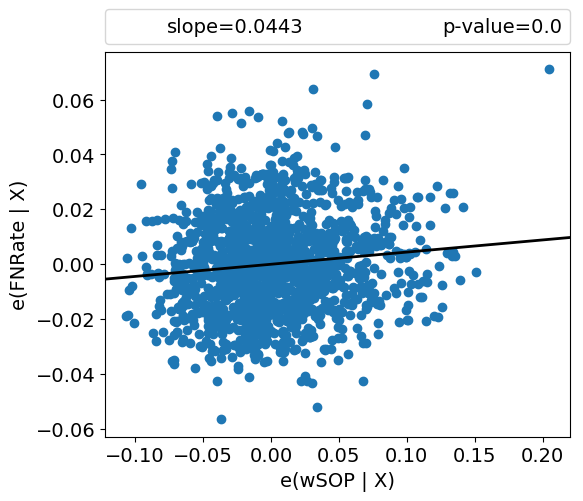
\includegraphics[width=0.22\textwidth]{Figure/NumGaps_SOP_TC_wSOP/precomputedInit/R4/fig/wsop_partial_regression}}
			\\\hline
			\rotatebox[origin=c]{-90}{R9} &
			\raisebox{-.5\height}{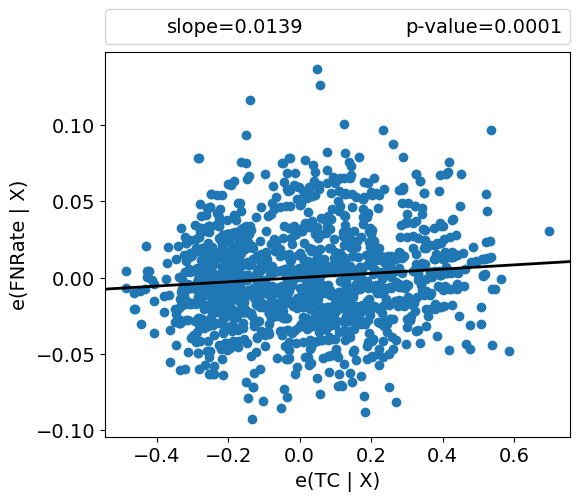
\includegraphics[width=0.22\textwidth]{Figure/NumGaps_SOP_TC_wSOP/precomputedInit/R9/fig/tc_partial_regression}} &
			\raisebox{-.5\height}{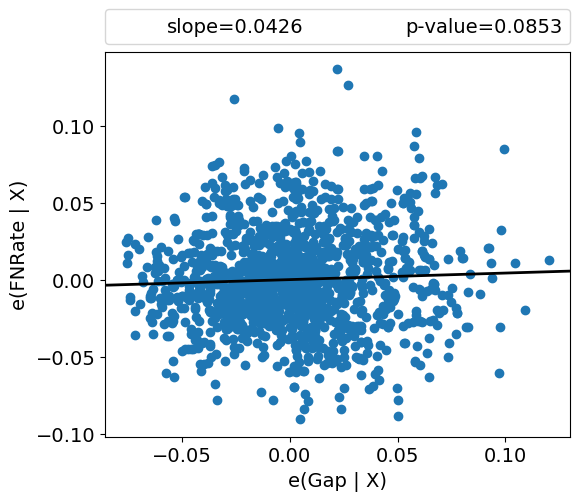
\includegraphics[width=0.22\textwidth]{Figure/NumGaps_SOP_TC_wSOP/precomputedInit/R9/fig/gap_partial_regression}} & 
			\raisebox{-.5\height}{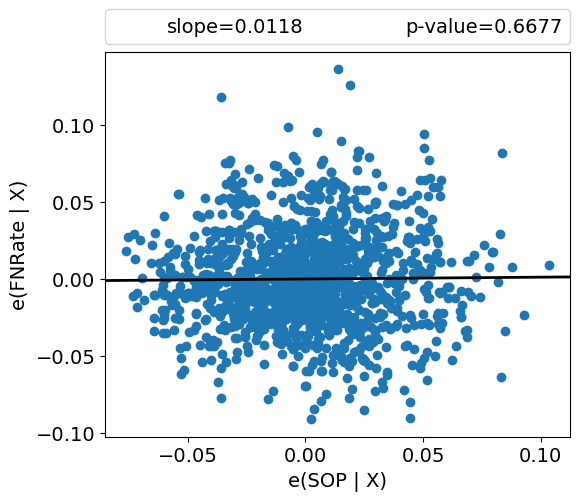
\includegraphics[width=0.22\textwidth]{Figure/NumGaps_SOP_TC_wSOP/precomputedInit/R9/fig/sop_partial_regression}} & 
			\raisebox{-.5\height}{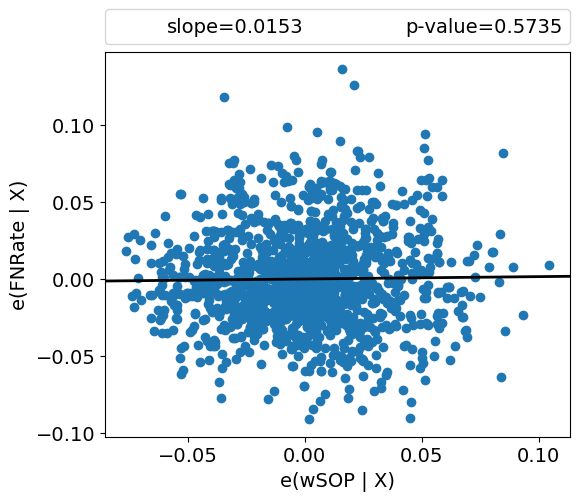
\includegraphics[width=0.22\textwidth]{Figure/NumGaps_SOP_TC_wSOP/precomputedInit/R9/fig/wsop_partial_regression}}
			\\\hline
			\rotatebox[origin=c]{-90}{R14} &
			\raisebox{-.5\height}{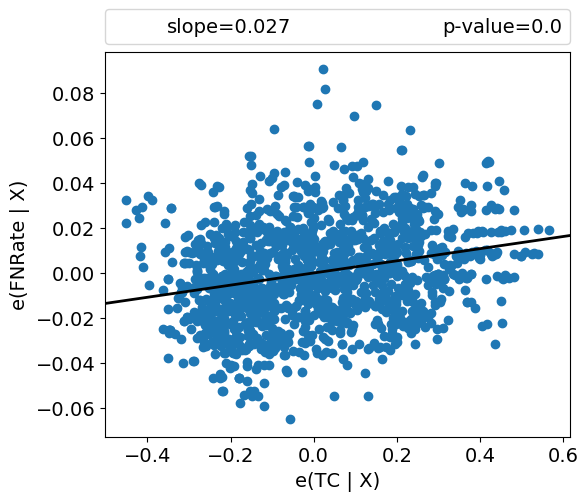
\includegraphics[width=0.22\textwidth]{Figure/NumGaps_SOP_TC_wSOP/precomputedInit/R14/fig/tc_partial_regression}} &
			\raisebox{-.5\height}{\includegraphics[width=0.22\textwidth]{Figure/NumGaps_SOP_TC_wSOP/precomputedInit/R14/fig/gap_partial_regression}} & 
			\raisebox{-.5\height}{\includegraphics[width=0.22\textwidth]{Figure/NumGaps_SOP_TC_wSOP/precomputedInit/R14/fig/sop_partial_regression}} & 
			\raisebox{-.5\height}{\includegraphics[width=0.22\textwidth]{Figure/NumGaps_SOP_TC_wSOP/precomputedInit/R14/fig/wsop_partial_regression}}
			\\\hline
			\rotatebox[origin=c]{-90}{R19} &
			\raisebox{-.5\height}{\includegraphics[width=0.22\textwidth]{Figure/NumGaps_SOP_TC_wSOP/precomputedInit/R19/fig/tc_partial_regression}} &
			\raisebox{-.5\height}{\includegraphics[width=0.22\textwidth]{Figure/NumGaps_SOP_TC_wSOP/precomputedInit/R19/fig/gap_partial_regression}} & 
			\raisebox{-.5\height}{\includegraphics[width=0.22\textwidth]{Figure/NumGaps_SOP_TC_wSOP/precomputedInit/R19/fig/sop_partial_regression}} & 
			\raisebox{-.5\height}{\includegraphics[width=0.22\textwidth]{Figure/NumGaps_SOP_TC_wSOP/precomputedInit/R19/fig/wsop_partial_regression}}
			\\\hline
		\end{tabular}
		\caption[Multiple linear regression model with objective functions from literature for 100-taxon simulated dataset]{\underline{100-taxon simulated dataset:} Multiple linear regression model for identifying the association among FN rate and three objective functions (TC, Gap and SOP/wSOP) fitted to five randomly selected replicates. There is one figure for each possible combination (replicate, objective function). Each partial regression plot shows the association between an objective function and FN rate while holding the remaining two objectives constant. In a plot for an objective function $ OF $, the horizontal axis, $e(OF|X)$, denotes the residuals from regressing $OF$ against the remaining objective functions and the vertical axis, $e(FNRate|X)$, denotes the residuals from regressing FN rate against all the objective functions except $ OF $.} 
		\label{fig:mul_lin_reg}
	\end{adjustwidth}
\end{figure*}

\begin{figure*}[!htbp]
	\centering
	%\begin{adjustwidth}{-1cm}{-1cm}
	\begin{subfigure}{0.32\textwidth}
		\includegraphics[width=\textwidth]{Figure/summary/precomputedInit/R0/objset_fnrate_rank}
		\caption{R0}
		%\label{fig:con_pr09}
	\end{subfigure}	
	\begin{subfigure}{0.32\textwidth}
		\includegraphics[width=\columnwidth]{Figure/summary/precomputedInit/R4/objset_fnrate_rank}
		\caption{R4}
		%\label{fig:con_pr09}
	\end{subfigure}
	\begin{subfigure}{0.32\textwidth}
		\includegraphics[width=\columnwidth]{Figure/summary/precomputedInit/R9/objset_fnrate_rank}
		\caption{R9}
		%\label{fig:con_pr09}
	\end{subfigure}
	
	\begin{subfigure}{0.32\textwidth}
		\includegraphics[width=\columnwidth]{Figure/summary/precomputedInit/R14/objset_fnrate_rank}
		\caption{R14}
		%\label{fig:con_pr09}
	\end{subfigure}
	\begin{subfigure}{0.32\textwidth}
		\includegraphics[width=\columnwidth]{Figure/summary/precomputedInit/R19/objset_fnrate_rank}
		\caption{R19}
		%\label{fig:con_pr09}
	\end{subfigure}
	\caption{\underline{100-taxon simulated dataset:} Comparison among objective sets based on the distribution of the collection of the best FN rates from each run. The performance of the state-of-the-art tools are shown using horizontal lines.}
	\label{fig:rank_best_fn_rate}
	%	\end{adjustwidth}
\end{figure*}


\begin{figure*}[!htbp]	
	\begin{adjustwidth}{-1cm}{-1cm}
		\centering
		\begin{subfigure}{0.35\textwidth}
			\includegraphics[width=\columnwidth]{Figure/6-obj-old/R0/fig/scatter_mattrix}
			\caption{R0}
			%\label{fig:con_pr09}
		\end{subfigure}	
		\begin{subfigure}{0.35\textwidth}
			\includegraphics[width=\columnwidth]{Figure/6-obj-old/R4/fig/scatter_mattrix}
			\caption{R4}
			%\label{fig:con_pr09}
		\end{subfigure}
		\begin{subfigure}{0.35\textwidth}
			\includegraphics[width=\columnwidth]{Figure/6-obj-old/R9/fig/scatter_mattrix}
			\caption{R9}
			%\label{fig:con_pr09}
		\end{subfigure}
		\begin{subfigure}{0.35\textwidth}
			\includegraphics[width=\columnwidth]{Figure/6-obj-old/R14/fig/scatter_mattrix}
			\caption{R14}
			%\label{fig:con_pr09}
		\end{subfigure}
		\begin{subfigure}{0.35\textwidth}
			\includegraphics[width=\columnwidth]{Figure/6-obj-old/R19/fig/scatter_mattrix}
			\caption{R19}
			%\label{fig:con_pr09}
		\end{subfigure}
		\caption[Scatter-plot matrices for six objective functions on 100-taxon simulated dataset]{\underline{100-taxon simulated dataset:} Scatter-plot matrices depicting the pairwise relationship of all objective functions on five randomly selected replicates. We turn each objective function into minimization form and then normalize using min-max technique. In each matrix, the diagonal cells show the distribution of objective values (estimated using kernel density estimation which is a non-parametric way to estimate the probability density function of a random variable) while the non-diagonal cells show the correlation between pairs of objective functions. Each upper-diagonal cell contains the value of correlation coefficient $r$ of the corresponding pair of objective functions.}
		\label{fig:new_nature_obj}
	\end{adjustwidth}
\end{figure*}
\begin{figure*}[!htbp]
	\centering
	\small
	\begin{adjustwidth}{-1cm}{-1cm}
		\begin{tabular}{l||C{0.24\textwidth}|C{0.24\textwidth}|C{0.24\textwidth}|C{0.24\textwidth} }
			& Entropy & GapCon & SimG & SimNG\\\hline\hline
			\rotatebox[origin=c]{-90}{R0} & 
			\raisebox{-.5\height}{\includegraphics[width=0.22\textwidth]{Figure/6-obj-old/precomputedInit/R0/fig/Entropy_partial_regression}} &
			\raisebox{-.5\height}{\includegraphics[width=0.22\textwidth]{Figure/6-obj-old/precomputedInit/R0/fig/GapCon_partial_regression}} & 
			\raisebox{-.5\height}{\includegraphics[width=0.22\textwidth]{Figure/6-obj-old/precomputedInit/R0/fig/SimG_partial_regression}} & 
			\raisebox{-.5\height}{\includegraphics[width=0.22\textwidth]{Figure/6-obj-old/precomputedInit/R0/fig/SimNG_partial_regression}} 	
			\\\hline
			\rotatebox[origin=c]{-90}{R4} &
			\raisebox{-.5\height}{\includegraphics[width=0.22\textwidth]{Figure/6-obj-old/precomputedInit/R4/fig/Entropy_partial_regression}} &
			\raisebox{-.5\height}{\includegraphics[width=0.22\textwidth]{Figure/6-obj-old/precomputedInit/R4/fig/GapCon_partial_regression}} & 
			\raisebox{-.5\height}{\includegraphics[width=0.22\textwidth]{Figure/6-obj-old/precomputedInit/R4/fig/SimG_partial_regression}} & 
			\raisebox{-.5\height}{\includegraphics[width=0.22\textwidth]{Figure/6-obj-old/precomputedInit/R4/fig/SimNG_partial_regression}}
			\\\hline
			\rotatebox[origin=c]{-90}{R9} &
			\raisebox{-.5\height}{\includegraphics[width=0.22\textwidth]{Figure/6-obj-old/precomputedInit/R9/fig/Entropy_partial_regression}} &
			\raisebox{-.5\height}{\includegraphics[width=0.22\textwidth]{Figure/6-obj-old/precomputedInit/R9/fig/GapCon_partial_regression}} & 
			\raisebox{-.5\height}{\includegraphics[width=0.22\textwidth]{Figure/6-obj-old/precomputedInit/R9/fig/SimG_partial_regression}} & 
			\raisebox{-.5\height}{\includegraphics[width=0.22\textwidth]{Figure/6-obj-old/precomputedInit/R9/fig/SimNG_partial_regression}}
			\\\hline
			\rotatebox[origin=c]{-90}{R14} &
			\raisebox{-.5\height}{\includegraphics[width=0.22\textwidth]{Figure/6-obj-old/precomputedInit/R14/fig/Entropy_partial_regression}} &
			\raisebox{-.5\height}{\includegraphics[width=0.22\textwidth]{Figure/6-obj-old/precomputedInit/R14/fig/GapCon_partial_regression}} & 
			\raisebox{-.5\height}{\includegraphics[width=0.22\textwidth]{Figure/6-obj-old/precomputedInit/R14/fig/SimG_partial_regression}} & 
			\raisebox{-.5\height}{\includegraphics[width=0.22\textwidth]{Figure/6-obj-old/precomputedInit/R14/fig/SimNG_partial_regression}}
			\\\hline
			\rotatebox[origin=c]{-90}{R19} &
			\raisebox{-.5\height}{\includegraphics[width=0.22\textwidth]{Figure/6-obj-old/precomputedInit/R19/fig/Entropy_partial_regression}} &
			\raisebox{-.5\height}{\includegraphics[width=0.22\textwidth]{Figure/6-obj-old/precomputedInit/R19/fig/GapCon_partial_regression}} & 
			\raisebox{-.5\height}{\includegraphics[width=0.22\textwidth]{Figure/6-obj-old/precomputedInit/R19/fig/SimG_partial_regression}} & 
			\raisebox{-.5\height}{\includegraphics[width=0.22\textwidth]{Figure/6-obj-old/precomputedInit/R19/fig/SimNG_partial_regression}}
			\\\hline
		\end{tabular}	
		\caption[Multiple linear regression model with our prorposed objective functions for 100-taxon simulated dataset]{\underline{100-taxon simulated dataset:} Multiple linear regression model for identifying the association among FN rate and three objective functions (SimNG, GapCon and SimG/Entropy) fitted to five randomly selected replicates. There is one figure for each possible combination (replicate, objective function). Each partial regression plot shows the association between an objective function and FN rate while holding the remaining two objectives constant.  In a plot for an objective function $ OF $, the horizontal axis, $e(OF|X)$, denotes the residuals from regressing $OF$ against the remaining objective functions and the vertical axis, $e(FNRate|X)$, denotes the residuals from regressing FN rate against all the objective functions except $ OF $.}
		\label{fig:new_mul_lin_reg}
	\end{adjustwidth}
\end{figure*}

\subsection{Evaluation of selected MO formulations}\label{sec:eval_formulation}Now we examine the efficacy of our chosen formulations (i.e., \{SimG, SimNG\} and \{Gap, SOP\}) based on two biological rRNA datasets and 27 BAliBASE instances. To accomplish this we conduct several repeated runs of NSGA-II on these datasets. Then we examine the generated alignments based on the alignment quality as well as based on the resultant phylogenetic trees.

\subsubsection{Results achieved on biological rRNA datasets}
\begin{figure*}[!htbp]
	\centering
	\begin{adjustwidth}{-0.5cm}{-0.5cm}
		\begin{subfigure}[b]{0.25\textwidth}
			\includegraphics[width=\columnwidth]{Figure/summary/precomputedInit/23S.E/fnrate_density_single_run}
			\caption{23S.E}
\end{subfigure}    
		\begin{subfigure}[b]{0.25\textwidth}
			\includegraphics[width=\columnwidth]{Figure/summary/precomputedInit/23S.E.aa_ag/fnrate_density_single_run}
			\caption{23S.E.aa\_ag}
\end{subfigure}
		\begin{subfigure}[b]{0.25\textwidth}
			\includegraphics[width=\columnwidth]{Figure/summary/precomputedInit/23S.E/objset_fnrate_rank}
			\caption{23S.E}
\end{subfigure}    
		\begin{subfigure}[b]{0.25\textwidth}
			\includegraphics[width=\columnwidth]{Figure/summary/precomputedInit/23S.E.aa_ag/objset_fnrate_rank}
			\caption{23S.E.aa\_ag}
\end{subfigure}
\begin{subfigure}{0.25\textwidth}
			\includegraphics[width=\columnwidth]{Figure/summary/precomputedInit/23S.E/tc_density_single_run}
			\caption{23S.E}
\end{subfigure}    
		\begin{subfigure}{0.25\textwidth}
			\includegraphics[width=\columnwidth]{Figure/summary/precomputedInit/23S.E.aa_ag/tc_density_single_run}
			\caption{23S.E.aa\_ag}
\end{subfigure}
		\begin{subfigure}{0.25\textwidth}
			\includegraphics[width=\columnwidth]{Figure/summary/precomputedInit/23S.E/objset_tc_rank}
			\caption{23S.E}
\end{subfigure}    
		\begin{subfigure}{0.25\textwidth}
			\includegraphics[width=\columnwidth]{Figure/summary/precomputedInit/23S.E.aa_ag/objset_tc_rank}
			\caption{23S.E.aa\_ag}
\end{subfigure}
\begin{subfigure}{0.25\textwidth}
			\includegraphics[width=\columnwidth]{Figure/summary/precomputedInit/23S.E/pairs_density_single_run}
			\caption{23S.E}
\end{subfigure}    
		\begin{subfigure}{0.25\textwidth}
			\includegraphics[width=\columnwidth]{Figure/summary/precomputedInit/23S.E.aa_ag/pairs_density_single_run}
			\caption{23S.E.aa\_ag}
\end{subfigure}
		\begin{subfigure}{0.25\textwidth}
			\includegraphics[width=\columnwidth]{Figure/summary/precomputedInit/23S.E/objset_pairs_rank}
			\caption{23S.E}
\end{subfigure}    
		\begin{subfigure}{0.25\textwidth}
			\includegraphics[width=\columnwidth]{Figure/summary/precomputedInit/23S.E.aa_ag/objset_pairs_rank}
			\caption{23S.E.aa\_ag}
\end{subfigure}
\begin{subfigure}{0.26\textwidth}
			\includegraphics[width=\columnwidth]{Figure/summary/precomputedInit/23S.E/fnrate_vs_tc}
			\caption{23S.E}
\end{subfigure}    
		\begin{subfigure}{0.26\textwidth}
			\includegraphics[width=\columnwidth]{Figure/summary/precomputedInit/23S.E.aa_ag/fnrate_vs_tc}
			\caption{23S.E.aa\_ag}
\end{subfigure}
		\begin{subfigure}{0.26\textwidth}
			\includegraphics[width=\columnwidth]{Figure/summary/precomputedInit/23S.E/fnrate_vs_sp}
			\caption{23S.E}
\end{subfigure}    
		\begin{subfigure}{0.26\textwidth}
			\includegraphics[width=\columnwidth]{Figure/summary/precomputedInit/23S.E.aa_ag/fnrate_vs_sp}
			\caption{23S.E.aa\_ag}
\end{subfigure}
	
	\caption[Results on biological rRNA datasets]{\underline{Results on biological rRNA datasets:} \textbf{Panel 1 (Top Panel):} part (a) and part (b) show the FN rates yielded from 100 final population members averaged across 10 independent executions of NSGA-II. Before averaging, we sort the 100 FN rates obtained per run. Next we calculate the average of the best FN rates acquired from 10 executions. We repeat this for the second best FN rates and so on.
		part (c) and part (d) show the variation of the best FN rates obtained across 10 runs using boxplots.  \textbf{Panel 2 (Panel 3):} part (e) and part (f) (part (i) and part (j)) show the 100 TC scores (SP scores) averaged across 10 executions. 
part (g) and part (h) (part (k) and part (l)) show the variations of the best TC (SP) scores collected from 10 executions.
\textbf{Panel 4 (Bottom panel):} part (m) and part (n) show the relationship between TC score and FN rate for various alignments. part (o) and part (p) show the relationship between SP score and FN rate. In each panel, the score achieved by nine MSA methods are shown using horizontal dashed lines.
	}
	\label{fig:fn_rate_tc_sp_bio}
\end{adjustwidth}
\end{figure*}
We have run NSGA-II (10 independent runs) optimizing our two selected objective sets on two datasets (23S.E \& 23S.E.aa\_ag). 
We report the performance comparison of the MO formulations against the nine state of the art tools in terms of FN rate in Figure~\ref{fig:fn_rate_tc_sp_bio} (top panel). Here, part (a) and part (b) show the FN rate obtained from 100 alignments (i.e., members of the final population) averaged across 10 runs. To get these averaged FN rates, we sort the FN rates 100 solutions generated per run in ascending order. Next we calculate the average of the lowest FN rates acquired from all of these runs. We repeat this for the second lowest ones and so on. These figures (part (a) and (b)) demonstrate a promising aspect of MO approach that for each data it can generate a substantial number of solutions that are superior than the outputs of state-of-the-art tools. However, a practitioner would be interested in the best solutions. Therefore, we summarize the best FN rate over 10 runs in part (c) and (d). For both datasets, we see that, among the nine tools, FSA performed the best, followed by PRANK in 23.S.E dataset and PASTA in 23S.E.aa\_ag dataset. The two MO formulations yielded improved FN rates compared to FSA in 23S.E.aa\_ag dataset (part (b) and part (d)). In fact, on average, the optimization of \{Gap, SOP\} produces around 10\% (40\%) solutions that are superior to FSA (PASTA) as illustrated in part (b). On the contrary, the set \{SimG, SimNG\}, while produces around 40\% solutions that are better than PASTA on average, is able to produce very few solutions that are better than FSA. As can be noticed from Part (d), \{Gap, SOP\} is able to consistently outperform the best tool (i.e., FSA) and in almost 40\% of the total runs, \{SimG, SimNG\} also outperforms FSA . Now we focus on the results for 23S.E dataset (part (a) and (c)).  In this case, both \{Gap, SOP\} and \{SimG, SimNG\} remain below the best (FSA) but above the second best (PRANK) tool by generating around 5\% solutions better than the latter.


We similarly analyze SP and TC scores and illustrate the results in Figure~\ref{fig:fn_rate_tc_sp_bio}. Evidently, the alignments generated by MO formulations, according to the two popular above-mentioned measures, could not outperform the best performing tool, PASTA.
Panel 4 of Figure~\ref{fig:fn_rate_tc_sp_bio} clearly illustrates the discrepancy between TC (SP) score and FN rate; please check part (m) and part (n) (part (o) and part (p)).
To summarize, the MSA methods exhibiting superiority than our MO formulations with respect to the widely accepted measures cannot attain better phylogenetic trees than our MO formulations (Panel 4 of Figure~\ref{fig:fn_rate_tc_sp_bio}). To elaborate, our objective sets have generated several alignments with lower (i.e., worse) TC scores than PASTA, which is the best performer among the nine state of the art tools according to TC score.  
Contrastingly however, these alignments have produced better phylogenetic trees (i.e., trees having better FN rates) than those tools. Moreover we witness discordance between FN rate and TC score from among the tools: while PASTA is the best performer in terms of the latter, it is in fact behind FSA in terms of the former. Similarly, a quick check of the comparison between SP score and FN rate illustrated in part (o) and part (p) of Panel 4 reveals that there are several alignments generated by the MO formulations with worse SP score than PASTA; however, trees produced by these alignments achieve better FN rates than that tool.   

\begin{table}[!h]
\centering
	\caption{Comparison of 100 solutions generated by one execution of NSGA-II with exis MSA ting nine MSA methods in terms of FN rate.} \includegraphics[width=0.5\columnwidth]{Figure/comparison_gap_sop}
	\label{tab:balibase_good_solutions}\end{table}




\begin{figure*}[!htbp]
	\begin{adjustwidth}{-1cm}{-1cm}
		\centering
		\begin{subfigure}[b]{0.26\textwidth}
			\includegraphics[width=\columnwidth]{Figure/summary/precomputedInit/Balibase/BB11005_fnrate_density_single_run}
			\caption{BB11005}
\end{subfigure}    
		\begin{subfigure}[b]{0.26\textwidth}
			\includegraphics[width=\columnwidth]{Figure/summary/precomputedInit/Balibase/BB11018_fnrate_density_single_run}
			\caption{BB11018}
\end{subfigure}
		\begin{subfigure}[b]{0.26\textwidth}
			\includegraphics[width=\columnwidth]{Figure/summary/precomputedInit/Balibase/BB11020_fnrate_density_single_run}
			\caption{BB11020}
\end{subfigure}
		\begin{subfigure}[b]{0.26\textwidth}
			\includegraphics[width=\columnwidth]{Figure/summary/precomputedInit/Balibase/BB11033_fnrate_density_single_run}
			\caption{BB11033}
\end{subfigure}
\begin{subfigure}{0.26\textwidth}
			\includegraphics[width=\columnwidth]{Figure/summary/precomputedInit/Balibase/BB11005_objset_fnrate_rank}
			\caption{BB11005}
\end{subfigure}    
		\begin{subfigure}{0.26\textwidth}
			\includegraphics[width=\columnwidth]{Figure/summary/precomputedInit/Balibase/BB11018_objset_fnrate_rank}
			\caption{BB11018}
\end{subfigure}
		\begin{subfigure}{0.26\textwidth}
			\includegraphics[width=\columnwidth]{Figure/summary/precomputedInit/Balibase/BB11020_objset_fnrate_rank}
			\caption{BB11020}
\end{subfigure}
\begin{subfigure}{0.26\textwidth}
			\includegraphics[width=\columnwidth]{Figure/summary/precomputedInit/Balibase/BB11033_objset_fnrate_rank}
			\caption{BB11033}
\end{subfigure}
		
\begin{subfigure}{0.26\textwidth}
			\includegraphics[width=\columnwidth]{Figure/summary/precomputedInit/Balibase/BB11005_fnrate_vs_tc_2}
			\caption{BB11005}
\end{subfigure}    
		\begin{subfigure}{0.26\textwidth}
			\includegraphics[width=\columnwidth]{Figure/summary/precomputedInit/Balibase/BB11018_fnrate_vs_tc_2}
			\caption{BB11018}
\end{subfigure}
		\begin{subfigure}{0.26\textwidth}
			\includegraphics[width=\columnwidth]{Figure/summary/precomputedInit/Balibase/BB11020_fnrate_vs_tc_2}
			\caption{BB11020}
\end{subfigure}
		\begin{subfigure}{0.26\textwidth}
			\includegraphics[width=\columnwidth]{Figure/summary/precomputedInit/Balibase/BB11033_fnrate_vs_tc_2}
			\caption{BB11033}
\end{subfigure}    
		\begin{subfigure}{0.26\textwidth}
			\includegraphics[width=\columnwidth]{Figure/summary/precomputedInit/Balibase/BB11005_fnrate_vs_sp_2}
			\caption{BB11005}
\end{subfigure}    
		\begin{subfigure}{0.26\textwidth}
			\includegraphics[width=\columnwidth]{Figure/summary/precomputedInit/Balibase/BB11018_fnrate_vs_sp_2}
			\caption{BB11018}
\end{subfigure}
		\begin{subfigure}{0.26\textwidth}
			\includegraphics[width=\columnwidth]{Figure/summary/precomputedInit/Balibase/BB11020_fnrate_vs_sp_2}
			\caption{BB11020}
\end{subfigure}
		\begin{subfigure}{0.26\textwidth}
			\includegraphics[width=\columnwidth]{Figure/summary/precomputedInit/Balibase/BB11033_fnrate_vs_sp_2}
			\caption{BB11033}
\end{subfigure}
	
	\caption[Results on RV11 based on tree quality]{ \underline{Results on RV11 based on tree quality:} \textbf{Panel 1 (Top panel):} part (a) - (d) show the averaged 100 (i.e., population size) FN rates obtained across 20 repeated executions of NSGA-II. 
\textbf{Panel 2:} part (e) - (h) show the variation of best FN rates accumulated from 20 repeated executions using boxplots. 
	\textbf{Panel 3 (Panel 4):} part (i) - (l) (part (m) - (p)) show the relationship between TC score (SP score) and FN rate obtained from various alignments. In each panel, FN rates attained by the existing MSA tools are shown using horizontal dashed lines.}
	\label{fig:rv11_fn_rate_tc_sp}
\end{adjustwidth}
\end{figure*}


\begin{figure*}[!htbp]
	\begin{adjustwidth}{-1cm}{-1cm}
		\centering
		\begin{subfigure}[b]{0.26\textwidth}
			\includegraphics[width=\columnwidth]{Figure/summary/precomputedInit/Balibase/BB11005_tc_density_single_run_2}
			\caption{BB11005}
\end{subfigure}    
		\begin{subfigure}[b]{0.26\textwidth}
			\includegraphics[width=\columnwidth]{Figure/summary/precomputedInit/Balibase/BB11018_tc_density_single_run_2}
			\caption{BB11018}
\end{subfigure}
		\begin{subfigure}[b]{0.26\textwidth}
			\includegraphics[width=\columnwidth]{Figure/summary/precomputedInit/Balibase/BB11020_tc_density_single_run_2}
			\caption{BB11020}
\end{subfigure}
\begin{subfigure}[b]{0.26\textwidth}
			\includegraphics[width=\columnwidth]{Figure/summary/precomputedInit/Balibase/BB11033_tc_density_single_run_2}
			\caption{BB11033}
\end{subfigure}
		\begin{subfigure}{0.26\textwidth}
			\includegraphics[width=\columnwidth]{Figure/summary/precomputedInit/Balibase/BB11005_objset_tc_rank_2}
			\caption{BB11005}
\end{subfigure}    
		\begin{subfigure}{0.26\textwidth}
			\includegraphics[width=\columnwidth]{Figure/summary/precomputedInit/Balibase/BB11018_objset_tc_rank_2}
			\caption{BB11018}
\end{subfigure}
		\begin{subfigure}{0.26\textwidth}
			\includegraphics[width=\columnwidth]{Figure/summary/precomputedInit/Balibase/BB11020_objset_tc_rank_2}
			\caption{BB11020}
\end{subfigure}
\begin{subfigure}{0.26\textwidth}
			\includegraphics[width=\columnwidth]{Figure/summary/precomputedInit/Balibase/BB11033_objset_tc_rank_2}
			\caption{BB11033}
\end{subfigure}
		
\begin{subfigure}{0.26\textwidth}
			\includegraphics[width=\columnwidth]{Figure/summary/precomputedInit/Balibase/BB11005_pairs_density_single_run_2}
			\caption{BB11005}
\end{subfigure}    
		\begin{subfigure}{0.26\textwidth}
			\includegraphics[width=\columnwidth]{Figure/summary/precomputedInit/Balibase/BB11018_pairs_density_single_run_2}
			\caption{BB11018}
\end{subfigure}
		\begin{subfigure}{0.26\textwidth}
			\includegraphics[width=\columnwidth]{Figure/summary/precomputedInit/Balibase/BB11020_pairs_density_single_run_2}
			\caption{BB11020}
\end{subfigure}
\begin{subfigure}{0.26\textwidth}
			\includegraphics[width=\columnwidth]{Figure/summary/precomputedInit/Balibase/BB11033_pairs_density_single_run_2}
			\caption{BB11033}
\end{subfigure}
		\begin{subfigure}{0.26\textwidth}
			\includegraphics[width=\columnwidth]{Figure/summary/precomputedInit/Balibase/BB11005_objset_pairs_rank_2}
			\caption{BB11005}
\end{subfigure}    
		\begin{subfigure}{0.26\textwidth}
			\includegraphics[width=\columnwidth]{Figure/summary/precomputedInit/Balibase/BB11018_objset_pairs_rank_2}
			\caption{BB11018}
\end{subfigure}
		\begin{subfigure}{0.26\textwidth}
			\includegraphics[width=\columnwidth]{Figure/summary/precomputedInit/Balibase/BB11020_objset_pairs_rank_2}
			\caption{BB11020}
\end{subfigure}
\begin{subfigure}{0.26\textwidth}
			\includegraphics[width=\columnwidth]{Figure/summary/precomputedInit/Balibase/BB11033_objset_pairs_rank_2}
			\caption{BB11033}
\end{subfigure}
	\end{adjustwidth}
	\caption[Results on RV11 based on alignment quality]{\underline{Results on RV11 based on alignment quality:} \textbf{Panel 1 (Panel 3)}: part (a) - (d) (part (i) - (l)) shows the averaged 100 TC scores (SP scores) obtained across 20 repeated executions of NSGA-II. 
\textbf{Panel 2 (Panel 4)}: part (e) - (h) (part (m) - (p)) shows the variation of best TC scores (SP scores) accumulated from 20 20 repeated executions using boxplots. In each panel, the score attained by existing MSA tools are shown  using horizontal dashed lines.}
	\label{fig:rv11_tc_sp}
	
\end{figure*}

\begin{figure*}[!h]
	\begin{adjustwidth}{-1cm}{-1cm}
		\centering
		\begin{subfigure}[b]{0.25\textwidth}
			\includegraphics[width=\columnwidth]{Figure/tree/BB20010_true_tree}
			\caption{True tree}
\end{subfigure}    
		\begin{subfigure}[b]{0.25\textwidth}
			\includegraphics[width=\columnwidth]{Figure/tree/BB20010_simg_tree}
			\caption{NSGA-II$_{\text{\{SimG, SimNG\}}}$}
\end{subfigure}
		\begin{subfigure}[b]{0.25\textwidth}
			\includegraphics[width=\columnwidth]{Figure/tree/BB20010_gap_tree}
			\caption{NSGA-II$_{\text{\{Gap, SOP\}}}$}
\end{subfigure}
		\begin{subfigure}[b]{0.25\textwidth}
			\includegraphics[width=\columnwidth]{Figure/tree/BB20010_fsa_tree}
			\caption{FSA}
\end{subfigure}
	\end{adjustwidth}
	\caption{ True phylogenetic tree along with the best estimated trees yielded by the two selected MO formulations and FSA method for BB20010.}
	\label{fig:bb20010_trees}
\end{figure*}
\subsubsection{Results on BAliBASE datasets}
We performed 20 repeated runs of NSGA-II on 27 random instances of BAliBASE 3.0. Once again we analyze obtained solutions in terms of the quality measures of alignments and phylogenetic trees and observe that the better alignments according to popular alignment measures, do not necessarily yield better phylogenetic trees.
Due to space constraints, we present our core observations on four instances (BB11018, BB11005, BB11033 \& BB11020 ) under RV11 group in Figures \ref{fig:rv11_fn_rate_tc_sp} and \ref{fig:rv11_tc_sp}. We obtained similar results for the remaining groups (RV12 to RV50) (please see Section~\ref{sec:result_balibase} in the supplementary file). Figure \ref{fig:rv11_fn_rate_tc_sp}) summarizes our findings based on FN rate. If we check the Top panel (part (a) - (h)), we find that, throughout all the instances, the solutions generated by the two objective sets are either better or at least equivalent when compared to the solutions generated by the best tool.  
For BB11020, the objective set \{SimG, SimNG\} achieves 12\% FN rate as opposed to 50\%, achieved by the best tool- clearly, a huge improvement. In terms of TC score however, the two objective sets have been able to outperform all the tools only for BB11020 (part (a) - part (h) of Figure \ref{fig:rv11_tc_sp}), which is conflicting with our findings in terms of the FN rate. So again we witness the discrepancy between TC score and FN rate illustrated in part (i) - part (l) of Figure~\ref{fig:rv11_fn_rate_tc_sp}. On the other hand, Figure \ref{fig:rv11_tc_sp} depicts the results based on SP and TC scores. If we observe its Panel 1 (part (i) - (p)), we see similar disagreement between SP score and FN rate depicted in part (m) - part (p) of Figure~\ref{fig:rv11_fn_rate_tc_sp}. It is clearly evident from these figures that the best TC and/or SP scores may not necessarily imply the best FN rates. This phenomenon is also observed quite consistently across rest of the instances. This finding may be of vital importance for researchers and practitioners, who leverage MSA methods in phylogenetic applications, 

\begin{table*}[!h]
	\scriptsize
	\centering
	\caption{Friedman test and Holm's post-hoc procedure. \underline{Friedman's rank (Column 2):} Average rank (lower rank indicates better) of the MSA approaches. \underline{Holm's adjusted $p$-values (Columns 3, 4 and 5):} Significance of difference between the metaheuristics and the MSA methods.}
	\begin{tabular}{|l|r||c|c|c|}
		\hline
		\multicolumn{1}{|c|}{1} & \multicolumn{1}{c||}{2} & 3     & 4     & 5 \\
		\hline
		\multicolumn{1}{|c|}{\multirow{2}{*}{Method}} & \multirow{2}{*}{Friedman's Rank*} & \multicolumn{3}{c|}{Holm's adjusted $p$-value} \\
		\cline{3-5}      &  & \multicolumn{1}{l|}{NSGA-II$_{\text{\{SimG, SimNG\}}}$} & \multicolumn{1}{l|}{MOEA/D$_{\text{\{SimG, SimNG\}}}$} & \multicolumn{1}{l|}{NSGA-II$_{\text{\{Gap, SOP\}}}$} \\
		\hline
		NSGA-II$_{\text{\{SimG, SimNG\}}}$ & 2.4630 & -     & \multicolumn{1}{r|}{1.00000} & \multicolumn{1}{r|}{1.00000} \\
		\hline
		MOEA/D$_{\text{\{SimG, SimNG\}}}$ & 3.1852 & \multicolumn{1}{r|}{1.00000} & -     &  \multicolumn{1}{r|}{1.00000} \\
		\hline
		NSGA-II$_{\text{\{Gap, SOP\}}}$ & 3.4444 & \multicolumn{1}{r|}{1.00000} &    \multicolumn{1}{r|}{1.00000}   & - \\
		\hline
		ProbCons & 6.6667 & \multicolumn{1}{r|}{0.00086} & \multicolumn{1}{r|}{0.01593} & \multicolumn{1}{r|}{0.04100} \\
		\hline
		Clustal $\Omega$ & 7.2222 & \multicolumn{1}{r|}{0.00007} & \multicolumn{1}{r|}{0.00171} & \multicolumn{1}{r|}{0.00497} \\
		\hline
		MAFFT & 7.3148 & \multicolumn{1}{r|}{0.00004} & \multicolumn{1}{r|}{0.00118} & \multicolumn{1}{r|}{0.00344} \\
		\hline
		Kalign & 7.5556 & \multicolumn{1}{r|}{0.00001} & \multicolumn{1}{r|}{0.00041} & \multicolumn{1}{r|}{0.00126} \\
		\hline
		PASTA & 7.7222 & \multicolumn{1}{r|}{0.00001} & \multicolumn{1}{r|}{0.00019} & \multicolumn{1}{r|}{0.00063} \\
		\hline
		FSA   & 7.8333 & \multicolumn{1}{r|}{0.00000} & \multicolumn{1}{r|}{0.00012} & \multicolumn{1}{r|}{0.00039} \\
		\hline
		MUSCLE & 8.0370 & \multicolumn{1}{r|}{0.00000} & \multicolumn{1}{r|}{0.00004} & \multicolumn{1}{r|}{0.00015} \\
		\hline
		Clustal W & 8.2037 & \multicolumn{1}{r|}{0.00000} & \multicolumn{1}{r|}{0.00002} & \multicolumn{1}{r|}{0.00007} \\
		\hline
		RetAlign & 8.3519 & \multicolumn{1}{r|}{0.00000} & \multicolumn{1}{r|}{0.00001} & \multicolumn{1}{r|}{0.00003} \\
		\hline
		\hline
		*Statistic & 14.3760 & \multicolumn{3}{c|}{\multirow{2}{*}{N/A}} \\
		\cline{1-2}    *$p$-value & 0.0000 & \multicolumn{3}{c|}{} \\
		\hline
	\end{tabular}\label{tab:friedman_holm}\end{table*}



Table~\ref{tab:balibase_good_solutions} shows a comparison of the averaged 100 FN rates yielded through a single execution of NSGA-II by optimizing the formulation, \{Gap, SOP\} against the existing MSA methods in terms of FN rate for the BAliBASE datasets. It shows that, on most of the cases, the MO approach can yield better phylogenetic trees than all MSA methods. As an illustration, for BB20010 we show the true tree and the most accurate estimated trees yielded by the two selected MO formulations and FSA (performed best among the nine MSA methods) in Figure~\ref{fig:bb20010_trees}. We further conducted a comparative analysis between NSGA-II and MOEA/D while optimizing \{SimG, SimNG\}. However, due to space constraints, the results are reported in Table~\ref{tab:balibase_good_solutions_simg_simng} and ~\ref{tab:superior_solutions} of the supplementary file.




\subsubsection{Statistical tests}
Here we assess whether the observed improvements in terms of FN rate attained by the MO formulations over the nine  MSA tools are statistically significant.
We apply an appropriate statistical significance test on 27 BAliBASE instances. So we gather paired data using the FN rate attained for each of the (MSA method, instance) pairs. In case of our metaheuristics, the average of the best (i.e., lowest) FN rates obtained from 20 repeated executions is taken. Since our data do not comply with the assumption of homoscedasticity and normality, following the suggestion of~\cite{derrac2011practical}, we have applied, with 95\% confidence level, a series of nonparametric tests.  


We first perform a (nonparametric) test due to Friedman (popularly known as the Friedman Test). Thus we are able to rank (lower rank implies better) all the methods as reported in Column 2 of Table~\ref{tab:friedman_holm}. We notice that the MO approaches are clearly ahead of the existing MSA tools. Next, we follow Holm's post-hoc procedure and report the adjusted $p$-value that indicates the significance of the difference in the FN rate between two methods thereby complementing the Friedman test rankings. The adjusted $p$-values are presented Columns 3 to 5 of the same table. 
These values show that the observed difference (i.e., improved FN rates) between a MO approach and each of the nine MSA tools are statistically significant (adjusted $p$-value $\le$ 0.05).

\begin{table}[htbp]
	\centering
	\caption{Overall performance (worst: 0, best: 10) of our proposed methodology across six subgroups of BAliBASE datasets.}
	\begin{tabular}{|c|r|}
		\hline
		Group & \multicolumn{1}{l|}{Avg. Score} \\
		\hline
		RV11  & 4.25 \\
		\hline
		RV12  & 8.4 \\
		\hline
		RV20  & 3.4 \\
		\hline
		RV30  & 5.25 \\
		\hline
		RV40  & 8 \\
		\hline
		RV50  & 6 \\
		\hline
	\end{tabular}%
	\label{tab:insight_group}%
\end{table}%

\subsection{Biological Perspective}\label{sec:discussion}
% Table generated by Excel2LaTeX from sheet 'Sheet1'
Here we attempt to characterize the overall performance of our proposed methodology using a biological perspective. To accomplish this, using the values reported in Table~\ref{tab:superior_solutions}, we systematically score the overall performance (worst: 0, best: 10) of our approach on a particular dataset. Then we categorize 27 biological instances of BAliBASE benchmark into different groups based on following biological criteria further analyze the performance of our approach.
\begin{itemize}
	\item \underline{Family and similarity:} BAliBASE datasets are divided into six subgroups according to this criterion as we discussed in Section~\ref{subsec:balibase_stat}. Table~\ref{tab:insight_group} reports the average score of our approach on each group. From these data, we can observe that, while our approach works
	reasonably well across 
	all groups, it works best on RV12 (medium to divergent sequences, 20\%-40\% residue identity) and RV40 (sequences with large terminal N/C extensions) compared to other groups.
	
	%\item For R19, where we saw an unusual regression result, the objective sets perform worse compared to other replicates.
	\item \underline{Evolutionary distance:} A simple measure of evolutionary distance between two aligned sequences is p-distance. For an MSA of $N$ sequences, we get $N \choose 2$ p-distances. We use average p-distance and variance thereof to classify the 27 instances into three clusters (see Figure~\ref{fig:balibase_cluster}) and report the average score of our method per cluster in Table~\ref{tab:cluster}. This somewhat suggests that, on Cluster 2, our approach fares slightly better.
	
	
	
	%	\begin{itemize}
	%		\item{Average of p-distances:} A higher value of this measure means that most of the species with the alignment are distantly related. Usually such a dataset is harder to analyze (with regards to alignment and phylogeny construction) compared to the ones with relatively lower average p-distance. Table~\ref{tab:insight_avg} shows the performance from this perspective. It does not provide us a specific trend.
	%		
	%		\item{Variance of p-distances:} This shows us how the distances between different pair of species within the alignment vary. We do not observe a significant pattern here (Table~\ref{tab:insight_variance}) as well. 
	%
	%	\end{itemize}
\end{itemize} 

\begin{figure}[!htbp] 
	\centering
	%\begin{adjustwidth}{-0.2cm}{-0.2cm}
	\includegraphics[width=0.7\textwidth]{Figure/balibase_cluster}
	%\vspace{-0.6cm}
	\caption{Classification of BAliBASE datasets into three clusters based on p-distances.} 
	\label{fig:balibase_cluster}
	%\end{adjustwidth}
\end{figure}

\begin{table}[htbp]
	\centering
	\caption{Overall performance (worst: 0, best: 10) of our proposed methodology on BAliBASE datasets across three clusters based on p-distances.}
	\begin{tabular}{|c|r|}
		\hline
		Group & \multicolumn{1}{l|}{Avg. Score} \\
		\hline
		Cluster 1 & 5.8 \\
		\hline
		Cluster 2 & 6.41 \\
		\hline
		Cluster 3 & 4.25 \\
		\hline
	\end{tabular}%
	\label{tab:cluster}%
\end{table}%


%% Table generated by Excel2LaTeX from sheet 'Sheet1'
%\begin{table}[htbp]
%	\centering
%	\caption{Overall performance (worst: 0, best: 10) of our proposed methodology on BAliBASE datasets across four equispaced ranges of average p-distances.}
%	\begin{tabular}{|c|r|}
%		\hline
%		Average p-distance & \multicolumn{1}{l|}{Performance} \\
%		\hline
%		0.5327 - 0.6129 & 5.75 \\
%		\hline
%		0.6129 - 0.6932 & 7.71 \\
%		\hline
%		0.6932 - 0.7734 & 5.70 \\
%		\hline
%		0.7734 - 0.8537 & 4.50 \\
%		\hline
%	\end{tabular}%
%	\label{tab:insight_avg}%
%\end{table}%
%
%
%% Table generated by Excel2LaTeX from sheet 'Sheet1'
%\begin{table}[htbp]
%	\centering
%	\caption{Overall performance (worst: 0, best: 10) of our proposed methodology on BAliBASE datasets across four equispaced ranges of variance of p-distances.}
%	\begin{tabular}{|c|r|}
%		\hline
%		Variance of p-distance & \multicolumn{1}{l|}{Performance} \\
%		\hline
%		0.0009 - 0.0105 & 6.33 \\
%		\hline
%		0.0105 - 0.0200 & 5.89 \\
%		\hline
%		0.0200 - 0.0296 & 5.20 \\
%		\hline
%		0.0296 - 0.0391 & 6.00 \\
%		\hline
%	\end{tabular}%
%	\label{tab:insight_variance}%
%\end{table}%

\subsection{Running time}\label{sec:run}
As we are dealing with an offline optimization problem, the runtime is not a major concern in this study. Our multi-objective metaheuristics make an effort to generate improved MSAs for phylogeny estimation by evolving a set of candidate solutions. So depending on the size of the set of candidate solutions, our approach may exhibit higher running time than the state-of-the-art MSA tools; in fact, in our experiments, our approach does require a higher running time. Nonetheless, to put everything into context, here we report runtimes of our multi-objective approaches as well as MAFFT~\citep{katoh2002mafft} that can generate a competitive alignment within a very reasonable time~\citep{ashkenazy2018multiple}, keeping in mind that the former approach leverages some altered versions of the alignments output by the latter tools. Figure~\ref{fig:runtime_comp} summarizes the average runtimes for each group of BAliBASE datasets. It helps us to identify the differences in runtimes between a two objectives approach and a four objectives one, which would be informative to practitioners and method developers. From this figure, we see that the runtimes of the multi-objective approaches are at least 10 times higher than that of MAFFT. Overall, the set of nonparametric objectives \{SimG, SimNG\} exhibits the lowest runtime among the multi-objective approaches. In several cases (such as, RV12, RV20, RV30, RV40), \{SimG, SimNG\} runs more than 1.5 times faster than \{Gap, SOP\}. The calculation of Gap takes a longer period compared to other objectives due to the additional effort of reading the substitution table values continuously. The evaluation of objective functions have been shown in the literature~\citep{zambrano2017m2align} to be the main computational bottleneck for computing MSAs by multi-objective metaheuristics. Therefore, the inclusion of Gap as an objective can heavily affect the overall running time of any algorithm. Moreover, by comparing the runtimes of \{SimG, SimNG\} and \{Gap, SOP, SimG, SimNG\}, we find that the runtimes of multi-objective metaheuristics increase linearly in the number of objectives. And the increase in runtime of the four objectives approach is mostly due to Gap. This can encourage more research effort in this direction as adding appropriate objective would definitely increase the accuracy of a multi-objective approach.

Informatively, we ran the multi-objective metaheuristics on a server with Intel(R) Xeon(R) CPU E5-4617 @ 2.90GHz processor and 64GB of RAM. In Table~\ref{tab:time} (also see Figure \ref{fig:runtime_comp}), we give a rough estimate of the total computational time that we invested to derive our results.



\begin{figure}[!htbp] 
	\centering
	%\begin{adjustwidth}{-0.2cm}{-0.2cm}
	\includegraphics[width=0.5\textwidth]{Figure/balibase_runtime_comparison}
	%\vspace{-0.6cm}
	\caption{Average runtimes of multi-objective approaches and MAFFT for each group of BAliBASE datasets.} 
	\label{fig:runtime_comp}
	%\end{adjustwidth}
\end{figure}


%\subsection{Computational time}
\begin{table}[htbp]
	\small
	\centering
	\caption{Computational time invested to study the impact of multi-objective formualtion of MSA.}
	\begin{tabular}{|l|l|}
		\hline 
		\multicolumn{1}{|c|}{Dataset} & \multicolumn{1}{c|}{Total time (hours)} \\ 
		\hline 
		100-taxon simulated dataset &  1269.38\\ 
		\hline 
		Biological rRNA dataset &  311.64\\ 
		\hline 
		BAliBASE dataset &  45.88\\ 
		\hline 
	\end{tabular} 
	\label{tab:time}%
\end{table}%


\begin{comment}
\begin{tabular}{|l|r||r|r|}
\hline
\multicolumn{1}{|c|}{1} & \multicolumn{1}{c||}{2} & \multicolumn{1}{c|}{3} & \multicolumn{1}{c|}{4} \\
\hline
\multicolumn{1}{|c|}{\multirow{2}{*}{Method}} &  \multirow{2}{*}{Friedman's Rank*}  & \multicolumn{2}{c|}{Holm's adjusted $p$-value} \\
\cline{3-4}     &  & NSGA-II$_{\text{\{SimG, SimNG\}}}$ & NSGA-II$_{\text{\{Gap, SOP\}}}$ \\
\hline
NSGA-II$_{\text{\{SimG, SimNG\}}}$ & 2.2037 & \multicolumn{1}{c|}{~~~~~~~~~~~~~~~~~~~~-} & 0.46018 \\
\hline
NSGA-II$_{\text{\{Gap, SOP\}}}$ & 2.8704 & 0.46018 & \multicolumn{1}{c|}{~~~~~~~~~~~~~~~~-} \\
\hline
ProbCons & 5.7963 & 0.00014 & 0.00238 \\
\hline
Clustal $\Omega$ & 6.2963 & 0.00002 & 0.00044 \\
\hline
MAFFT & 6.4074 & 0.00001 & 0.00036 \\
\hline
Kalign & 6.7037 & 0.00000 & 0.00011 \\
\hline
PASTA & 6.8148 & 0.00000 & 0.00007 \\
\hline
FSA   & 6.9444 & 0.00000 & 0.00004 \\
\hline
MUSCLE & 7.1482 & 0.00000 & 0.00002 \\
\hline
Clustal W & 7.3519 & 0.00000 & 0.00001 \\
\hline
RetAlign & 7.4630 & 0.00000 & 0.00000 \\
\hline
\hline
\multicolumn{1}{|c|}{*Statistic} & 10.5911 & \multicolumn{2}{c|}{\multirow{2}{*}{N/A}} \\
\cline{1-2}    \multicolumn{1}{|c|}{*$p$-value} & 0.00000 & \multicolumn{2}{c|}{} \\
\hline
\end{tabular}\end{comment}

 \section{Conclusion} \label{sec:discussion}
We developed an application-oriented MO approach for computing MSAs for the purpose of phylogeny inference with the help of statistical techniques and domain knowledge. In addition to the existing objective functions for MSA, we introduced four simple ones. 
We applied multivariate linear regression in order to learn how an an individual objective function correlates with the FN rate, i.e., the fitness of the estimated phylogenetic tree. Thereby, we select two appropriate bi-objective formulations to move forward through empirical justification. Finally, by experimenting with simulated and biological datasets, we demonstrate that an application-aware MO formulation of MSA can guide us to improved phylogenetic trees compared to the existing MSA tools. This finding allow us to speculate that, domain-specific metrics can assist MSA methods for other application purposes also. 





\begin{comment}
MSAs are computed to serve various biological purposes including phylogeny estimation and protein structure prediction. The definition of what constitutes a correct alignment can depend partly on the purpose of MSAs~\citep{warnow2017computational}. Nevertheless, regardless of the purpose, the sites within the correct alignment define the ``homologies''. Therefore, homology can be based on structural features or evolutionary histories, leading to the opposing concepts of ``structural homology'' and ``evolutionary homology''~\citep{warnow2017computational}. While structural alignments are expected to be close to the true (evolutionary) alignment, convergent evolution may create conditions where the best structural alignment puts nucleotides or amino acids in the same site (thus implying homologies), even though these specific homologies are not present in the true evolutionary alignment~\citep{iantorno2014watches}. In other words, structural homology may not be identical to evolutionary homology~\citep{reeck1987homology}. In such a situation, generic metrics such as TC/SP score might not be adequate to assess the correctness of the estimated MSAs. Therefore, using more informative metrics (e.g. phylogeny as done in the study) to tailor adequate MO formulation of this problem seems a promising endeavor.

Standard criteria (SP score, TC score, etc.) for assessing alignment quality are usually based on shared homology pairs (SP score) or identical columns (TC score), and do not explicitly consider a particular application domain. Mistakes in alignments that are not important with respect to an application domain may not impact the ultimate accuracy of that particular inference. For example, not all sites are significant with respect to protein structure and function prediction, and hence multiple alignments with different accuracy may lead to the same predictions~\citep{warnow2013large}. Similarly, in the context of phylogeny estimation, alignments with substantially different SP scores may lead to trees with the same accuracy~\citep{liu2009rapid}. In this study, we systematically investigate the impact of evaluation criteria of an alignment on phylogenetic tree inference problem. Our results suggest that it could be possible to develop improved MSA methods for phylogenetic analysis by carefully choosing appropriate objective functions. Moreover, in almost all existing studies on MSA, we find the researchers evaluating the effectiveness of MSA methods using some generic alignment quality measures (i.e., TC score, SP score). Contrastingly, our results revealed that optimizing those widely used measures do not necessarily lead us to the best phylogenetic tree. This finding could be an eye opener for the researchers who need to use MSA methods to address a particular application. 

Our findings and proposed MO formulation can be particularly beneficial for iterative methods like SAT\'e and PASTA that iteratively co-estimate both alignment and tree. These methods obtain an initial alignment and a tree that guide each other to improved estimates in an iterative fashion. They make an effort to exploit the close association between the accuracy of an MSA and the corresponding tree in finding the output through multiple iterations from both directions. Therefore, carefully choosing an evaluation metric for an MSA with a better correlation to the tree accuracy seems likely to improve the results of these co-estimation techniques. Thus, our methodology, if adopted, may potentially have a profound positive impact on the accuracy of these iterative co-estimation techniques. Moreover, multiple ``good'' alignments from the output of the MO approach can be served as alternative MSAs for several methods (such as~\citep{ashkenazy2018multiple}) which would then utilize all of them to infer phylogeny with better accuracy.

This study will encourage the scientific community to investigate various application-aware measures for computing and evaluating MSAs. This will potentially prompt more experimental studies addressing specific application domains; and ultimately will propel our understanding of MSAs and their impact in various domains in computational biology, i.e, phylogeny estimation, protein structure and function prediction, orthology prediction etc. This study will also encourage the researchers to develop new scalable MSA tools by simultaneously optimizing multiple appropriate optimization criteria. Thus, we believe that this study will pioneer new models and optimization criteria for computing MSAs -- laying a firm, broad foundation for application specific MO formulation for estimating multiple sequence alignment.
\end{comment}
This study focus on devising a methodology for selecting an effective MO formulation by utilizing an application-aware measure.  Our methodology is applicable to the problems where an application-specific measure can be developed based on the ground truth provided by a dataset. In the future, we will employ recently developed MO algorithms (e.g.,~\cite{8981871, 9047876, 9097242}) to find out which one can give us the best performance. Currently, we are working to hybridize the MO approach with MUSCLE, a single-objective based MSA tool, leveraging the MOEA/D framework. Moreover, at present, we applied our methodology using the most common objective functions. We will include more existing objectives to highlight our findings. We conducted a comprehensive experimental study based on twenty nine datasets having various complexities and sizes, and our results and findings are conformable across all the datasets. Nevertheless, our methodology may be unable to perform satisfactorily on some MSA instances. In addition, at present, we did not make any attempt in improving the runtime of our MO approach which admittedly is computationally expensive than the popular MSA methods (please see Section~\ref{sec:run} of the supplementary file for some results and discussion). But it is possible to achieve enough speedup by utilizing advanced computing architectures as well as efficient implementation of core operations~\cite{8255834, 7738460}.  



